% =========================================================================
% Artigo IEEE Access — PID cascata x LQRy no drone hibrido (SIL + HIL)
% Estrutura definida por Kaue + orientadora; rascunho montado em 2026-08-02.
% Compilar: pdflatex main.tex (ou Overleaf). Classe: ieeeaccess.cls (inclusa).
% Marcadores [PENDENTE: ...] em vermelho = partes a completar (varias do Mirko).
% =========================================================================
\documentclass{ieeeaccess}
\usepackage{cite}
\usepackage{amsmath,amssymb,amsfonts}
\usepackage{graphicx}
\usepackage{textcomp}
\usepackage{booktabs}
\usepackage{url}
% tikz x ieeeaccess.cls: a carga do pgf emite 2 erros recuperados
% ("Missing number"/"Extra \fi", no submodulo random, que nao usamos).
% Atrito conhecido da classe; nao afeta o PDF — ignorar no log.
\usepackage{tikz}
\usetikzlibrary{arrows.meta,calc,positioning}
% Os titulos de secao usam a cor spot PANTONE3015C da classe, que sai
% INVISIVEL em varios visualizadores (Preview/poppler: "Bad color
% space"). Forca o azul IEEE Access equivalente em RGB.
\definecolor{accessblue}{RGB}{0,98,155}

% Compat: a classe so define \xfigwd dentro do macro \Figure{} dela; com
% ambientes figure padrao a caption falharia sem isto.
\makeatletter
\def\xfigwd{0pt}
\makeatother

% ---- marcador de pendencia (visivel em vermelho no PDF) ----
\newcommand{\pendente}[1]{\textcolor{red}{\textbf{[PENDENTE: #1]}}}
% ---- notacao ----
\newcommand{\VT}{V_T}
\graphicspath{{figs/}}

\begin{document}
\history{Draft — not submitted.}
\doi{}

\title{Cascade PID Versus Output-Feedback LQR for the Fixed-Wing Flight
Mode of a Hybrid VTOL UAV: Design, Robustness, and a Deterministic
Hardware-in-the-Loop Comparison}

% ---------------------------------------------------------------
% \pendente{confirmar e-mails e ORCIDs dos coautores}
\author{\uppercase{Kau\^e Martins}\authorrefmark{1},
\uppercase{Huascar Mirko Montecinos Cortez}\authorrefmark{1},
and \uppercase{Neusa Maria Franco de Oliveira}\authorrefmark{1}}
\address[1]{Instituto Tecnol\'ogico de Aeron\'autica (ITA), S\~ao Jos\'e dos
Campos, SP, Brazil (e-mail: kaue.martins124@gmail.com)}
\tfootnote{Source code and simulation data are available at
\underline{https://github.com/Kauemartinsxd/controle-pid-drone-hibrido}.}

\markboth
{Martins \headeretal: Cascade PID Versus Output-Feedback LQR for the Fixed-Wing Mode of a Hybrid VTOL UAV}
{Martins \headeretal: Cascade PID Versus Output-Feedback LQR for the Fixed-Wing Mode of a Hybrid VTOL UAV}

\corresp{Corresponding author: Kau\^e Martins (e-mail: kaue.martins124@gmail.com).}

\begin{abstract}
This article compares two flight control laws --- a classical cascade PID
and an output-feedback linear--quadratic regulator (LQRy) --- for the
fixed-wing flight mode of a small hybrid vertical take-off and landing
(VTOL) UAV, following the complete path from design to embedded
validation. Both controllers are designed on a model linearized about the
cruise trim of a nonlinear model identified from flight-test data, whose
open-loop dynamics include an unstable spiral mode, and are evaluated
against a common set of literature-grounded closed-loop requirements. In
software-in-the-loop (SIL) simulation on the nonlinear model, the two
laws are exercised under identical references on a 300-second combined
mission; the requirements-retuned PID meets every requirement and is
the tighter law on every guidance channel, while the deliberately soft
fixed-gain LQRy is slower, concedes up to a factor of five in RMS
tracking error, and violates the airspeed-overshoot requirement. A
robustness study then inverts that verdict: under a severe
lateral--directional model mismatch --- an independent identification
of the same airframe with sign-inverted lateral derivatives --- the
PID loses the mission outright, while the fixed-gain LQRy completes it
with near-nominal error --- a tolerance consistent with the classical
robustness heritage of LQ designs, though earned here by the soft
tuning. Under a longitudinal-only mismatch the LQRy stays nominal
and the PID's clamped altitude loop drifts; under wind and gusts both
complete the mission with the PID firmer; both tolerate a plausible
$+10\%$ identification uncertainty. Finally, both controllers are
deployed on an STM32 microcontroller through automatic code generation
and compared on a lockstep serial hardware-in-the-loop (HIL) bench
that is shown to be bit-deterministic and reproduces the SIL verdict,
with, for the synchronized PID deployment, a SIL--HIL residual at the
quantization floor of the bus, and a sensitivity study ranking the
implementation choices that actually affect embedded agreement. The
complete toolchain and data are publicly available.
\end{abstract}

\begin{keywords}
Cascade control, code generation, fixed-wing UAV, hardware-in-the-loop
simulation, hybrid VTOL aircraft, LQR control, PID control, robustness,
STM32.
\end{keywords}

\titlepgskip=-15pt
\maketitle

\section{Introduction}
\label{sec:introduction}

\PARstart{H}{ybrid} vertical take-off and landing (VTOL) aircraft
combine the hovering capability of multirotors with the range and
efficiency of fixed-wing flight, and have consequently become one of
the fastest-growing classes of unmanned aerial vehicles
(UAVs)~\cite{saeed2018survey,ducard2021review}. The price of this
versatility is a control problem that changes structure between flight
regimes, and the literature increasingly treats each regime as a
control problem in its own right~\cite{hu2024hybrid}. This article
focuses on the \emph{fixed-wing flight mode} of a hybrid VTOL platform
--- the mode in which the vehicle spends most of its mission --- and on
the complete path from controller design to embedded validation;
hover and transition are outside its scope.

\subsection{Related Work}
Autopilots for small UAVs remain dominated by nested
proportional--integral--derivative (PID) loops, a
legacy of their simplicity and field-proven
robustness~\cite{chao2010autopilots}, and this architecture underpins
the open-source flight stacks in widespread use
today~\cite{ebeid2018survey,meier2015px4}. Linear--quadratic (LQ)
methods are the natural model-based alternative, and comparisons
between the two families have accumulated since the seminal indoor
quadrotor study of Bouabdallah \emph{et
al.}~\cite{bouabdallah2004pid}: on quadrotor
platforms~\cite{argentim2013pid,rinaldi2023comparative}, on a
commercial mini-drone with experimental PID/LQR/MPC
benchmarks~\cite{okasha2022design}, and, less frequently, on
fixed-wing longitudinal dynamics~\cite{ingabire2019control}.

Hardware-in-the-loop (HIL) simulation --- preceded in practice by
software-in-the-loop (SIL) verification on the same models --- is the
established way to close the gap between simulation and flight: the embedded control system is
exercised against a simulated plant, so faults in the embedded
implementation surface on the bench rather than in the
air~\cite{jung2007hil,cai2009design}. The practice extends from
classical avionics benches to recent microcontroller-class autopilot
platforms~\cite{coopmans2015software,laabousse2025advanced}, is
integral to model-based development workflows in which the flight code
is generated automatically from the verified
model~\cite{erkkinen2006automatic,erkkinen2009model,paw2011integrated},
and has been applied to hybrid VTOL vehicles in the Brazilian research
context~\cite{silva2019control}. Within our research group, this
lineage runs through the Pegasus autopilot HIL
architecture~\cite{bittar2012pegasus}, X-Plane-based HIL of small-UAV
attitude control under atmospheric
disturbances~\cite{bittar2014hil}, and the bench-validated
fixed-wing autopilot of Santos~\cite{santos2018,santos2017hilloops},
whose cascade methodology this work adopts. The aircraft models in
this line of work are identified from flight-test
data~\cite{sato2021,sato2020identificacao,angelo2026}.

\subsection{Research Gaps}
Three gaps recur in this comparative literature:
\begin{enumerate}
  \item \emph{Platform.} Most PID--LQ comparisons target rotary-wing
        platforms; the fixed-wing mode of a hybrid VTOL vehicle is
        rarely the object of study.
  \item \emph{Mission-level embedded evaluation.} The comparisons are
        usually confined to simulation of isolated channels, rather
        than a full mission exercising the longitudinal and
        lateral--directional loops together on the embedded
        implementation.
  \item \emph{Robustness.} Arguably where the two design philosophies
        should differ most, robustness is seldom part of the
        protocol, even though LQ designs carry classical margin
        guarantees~\cite{safonov1977gain} that do not survive output
        feedback in general~\cite{doyle1978guaranteed}.
\end{enumerate}

\subsection{Contributions}
The present work addresses these gaps, extending the group lineage in
three directions: the plant
is the fixed-wing mode of a \emph{hybrid VTOL} aircraft rather than a
conventional fixed-wing one; the embedded controller is not hand-coded
but \emph{automatically generated} from the same Simulink model that
was verified in simulation, so that the tested artifact is the
production code itself; and two different control laws --- a cascade
PID and an output-feedback LQR (LQRy) --- are designed against a
common, literature-grounded requirements set, stressed under model
mismatch and wind, and deployed on the same bench under identical
conditions.

The main contributions of this work are:
\begin{itemize}
  \item the design of a cascade PID architecture for the fixed-wing
        flight mode of a hybrid VTOL aircraft, evaluated against a
        fixed-gain output-feedback LQR (LQRy) designed for the same
        platform, both judged against a common set of
        literature-grounded closed-loop requirements;
  \item a robustness study that inverts the nominal verdict: a
        severe, sign-changing lateral--directional model mismatch
        makes the aggressively tuned cascade PID lose the mission
        outright, while the soft fixed-gain LQRy completes it with
        near-nominal error --- with the remaining scenarios adding
        nuance: under a longitudinal-only mismatch the LQRy stays
        nominal while the PID's clamped altitude loop drifts, under
        wind and gusts the PID is the firmer law, and both tolerate a
        plausible $+10\%$ identification uncertainty;
  \item a low-cost HIL architecture based on
        automatic code generation and a lockstep serial protocol, whose
        SIL--HIL residual is shown to reach the quantization floor of
        the communication bus for the synchronized PID deployment;
  \item the characterization of the lockstep HIL loop as a
        \emph{deterministic} system --- demonstrated by bit-exact
        reproduction of full 300-second flight cases across two
        microcontroller models --- and its use to quantify how much each
        implementation choice affects SIL--HIL agreement; and
  \item a controlled, like-for-like comparison of the two controllers on
        the same rig, same references, and same metrics, with the known
        asymmetries of the two design harnesses disclosed explicitly.
\end{itemize}

\subsection{Organization}
Section~\ref{sec:model} presents the nonlinear model, the trim condition,
and the linearization. Section~\ref{sec:control} details the closed-loop
requirements and both controller designs. Section~\ref{sec:sil} reports
the SIL simulations and the controller comparison.
Section~\ref{sec:robustness} presents the robustness study.
Section~\ref{sec:hil} describes the HIL development, the determinism and
sensitivity analyses, and the embedded results.
Section~\ref{sec:conclusion} concludes the article.

\section{Nonlinear Model, Trim, and Linearization}
\label{sec:model}

\subsection{Nonlinear Model}
The aircraft is a small hybrid VTOL platform with a conventional
fixed-wing configuration for cruise. Its physical parameters are
$m=2.2$\,kg, wing area $S=0.27$\,m$^2$, span $b=1.2$\,m, mean aerodynamic
chord $\bar{c}=0.226$\,m (aspect ratio $AR=5.33$, Oswald factor $e=0.8$),
and inertia tensor (kg\,m$^2$)
\begin{equation}
\mathbf{I}=\begin{bmatrix}
0.1441 & 0 & -0.00167\\
0 & 0.1155 & 0\\
-0.00167 & 0 & 0.2572
\end{bmatrix}.
\end{equation}

The complete six-degree-of-freedom nonlinear model of this
aircraft~\cite{ferreira2019modeling,repo} follows the standard rigid-body
formulation~\cite{stevens2016aircraft} and is implemented in Simulink with a
state vector of 14 states (body velocities, angular rates, Euler angles,
and navigation states). The aerodynamic model uses the usual
coefficient build-up,
\begin{equation}
\begin{aligned}
C_L &= C_{L_0} + C_{L_\alpha}\alpha + C_{L_q}\frac{q\bar{c}}{2V_0}, \quad
C_D = C_{D_0} + \frac{C_L^2}{\pi e AR},\\
C_m &= C_{m_0} + C_{m_\alpha}\alpha + C_{m_{\delta_e}}\delta_e +
C_{m_q}\frac{q\bar{c}}{2V_0},
\end{aligned}
\end{equation}
with analogous expressions for the lateral--directional coefficients
$C_Y$, $C_l$, and $C_n$ in $\beta$, $p$, $r$, $\delta_a$, and $\delta_r$.
The stability and control derivatives were obtained by system
identification from flight-test data of the actual
aircraft~\cite{angelo2026} (longitudinal Model~4 and
lateral--directional Model~2 of that identification campaign),
following the time-domain output-error practice that is standard for
flight-vehicle identification~\cite{jategaonkar2006flight} and for
small UAVs in particular~\cite{dorobantu2012system}. Thrust is
modeled as $T = T_{max}\,\delta_t\,(\rho/\rho_0)^{0.8}$ with
$T_{max}=14$\,N.

In the fixed-wing flight mode considered here the hover rotors are
inactive, so the plant input vector comprises the four aerodynamic
commands and the three components of the wind velocity, the latter
expressed in the local NED frame:
\begin{equation}
\label{eq:inputvec}
U=[\,\underbrace{\delta_t\;\;\delta_e\;\;\delta_a\;\;\delta_r}_{\text{commands}}
\;\;|\;\;
\underbrace{w_N\;\;w_E\;\;w_D}_{\text{wind (NED)}}\,]^{\!\top}.
\end{equation}
The wind components are rotated into body axes and subtracted from the
inertial velocities before the aerodynamic triad is formed, so that
airspeed, angle of attack, and sideslip are computed from the
\emph{air-relative} velocity,
$V_T=\lVert[\,u\;v\;w\,]^{\!\top}-L_{bn}[\,w_N\;w_E\;w_D\,]^{\!\top}\rVert$,
in the usual way~\cite{stevens2016aircraft}. Wind therefore enters the model as a
physical disturbance input to the aerodynamics rather than as an additive
signal on the outputs; it is identically zero at trim and in the nominal
simulations, and is exercised as a disturbance in the robustness study of
Section~\ref{sec:robustness}.

Actuator dynamics are included explicitly, since the controllers are
ultimately deployed on hardware: each control surface is limited to
$\pm25^\circ$ in position and $150^\circ$/s in rate, followed by a
first-order lag of $\tau_{act}=0.05$\,s (20\,rad/s bandwidth); the
throttle channel is limited to $[0,1]$ with a rate limit of 1\,s$^{-1}$
and a spool-up lag of $\tau_{eng}=0.30$\,s. Without these, a reference
step produces an unrealizable impulsive surface deflection
(${\sim}400^\circ$/s in a single step) that no servo --- and no HIL
target --- could reproduce.

\subsection{Trim Condition}
\label{sec:trim}
The aircraft is trimmed numerically --- a Newton solution of
$\dot{x}=f(x,\delta)=0$ under the flight-condition constraints, the
standard formulation of the general aircraft trim
problem~\cite{marco2007trim,stevens2016aircraft} --- in
steady, wings-level horizontal flight at airspeed $\VT^e = 12.0$\,m/s,
altitude $h^e = 600$\,m, and flight-path angle $\gamma^e = 0$. The
resulting equilibrium is stated explicitly below, as it anchors every
simulation and every embedded test in this article.

\emph{State vector at trim} (body axes; unlisted states are zero):
\begin{equation}
\label{eq:xtrim}
\begin{aligned}
u^e &= 11.621~\text{m/s}, \quad
w^e = 2.992~\text{m/s}, \\
\theta^e &= 0.25196~\text{rad} = 14.44^\circ, \quad
h^e = 600~\text{m},
\end{aligned}
\end{equation}
so that $\VT^e=\sqrt{(u^e)^2+(w^e)^2}=12.0$\,m/s and, since
$\alpha^e=\arctan(w^e/u^e)=14.44^\circ=\theta^e$, the flight-path angle is
indeed $\gamma^e=\theta^e-\alpha^e=0$.

\emph{Output vector at trim}:
\begin{equation}
\label{eq:ytrim}
\VT^e = 12.0~\text{m/s},\;\;
\alpha^e = 14.44^\circ,\;\;
\beta^e = 0,\;\;
\gamma^e = 0,
\end{equation}
with $p^e=q^e=r^e=0$, $\phi^e=\psi^e=0$, $\theta^e=14.44^\circ$, and
$h^e=600$\,m.

\emph{Command vector at trim} (control surfaces and throttle):
\begin{equation}
\label{eq:dtrim}
\delta^e =
\begin{bmatrix}
\delta_{t}^{e} \\ \delta_{e}^{e} \\ \delta_{a}^{e} \\ \delta_{r}^{e}
\end{bmatrix}
=
\begin{bmatrix}
0.2836 \\ 0.1330~\text{rad}~(7.62^\circ) \\ 0 \\ 0
\end{bmatrix},
\end{equation}
with the hover-rotor commands identically zero in this flight mode.
Throughout the article, the controllers act on \emph{increments} around
this trim; the trim commands of~\eqref{eq:dtrim} are added at the
controller output (see the remark in Section~\ref{sec:sil-trim}).

\subsection{Linearization}
The nonlinear model is linearized about the trim
condition~\eqref{eq:xtrim}--\eqref{eq:dtrim}, decoupling into the standard
longitudinal and lateral--directional subsystems used for controller
design in Section~\ref{sec:control}. With longitudinal states
$x_{lon}=[\,u\;\alpha\;q\;\theta\;h\,]^{\!\top}$ and inputs
$[\,\delta_t\;\delta_e\,]^{\!\top}$:
\begin{equation}
\resizebox{.91\linewidth}{!}{$
A_{lon}=\begin{bmatrix}
0.124 & 13.29 & -2.643 & -9.497 & 0\\
-0.135 & -2.989 & 0.751 & 0 & 0\\
0 & -38.75 & -4.108 & 0 & 0\\
0 & 0 & 1 & 0 & 0\\
0 & -12 & 0 & 12 & 0
\end{bmatrix}\!,\;
B_{lon}=\begin{bmatrix}
6.071 & 0\\ -0.126 & 0\\ 0 & 45.98\\ 0 & 0\\ 0 & 0
\end{bmatrix}
$}
\end{equation}
and with lateral--directional states
$x_{lat}=[\,\beta\;p\;r\;\phi\;\psi\,]^{\!\top}$ and inputs
$[\,\delta_a\;\delta_r\,]^{\!\top}$:
\begin{equation}
\resizebox{.91\linewidth}{!}{$
A_{lat}=\begin{bmatrix}
-0.478 & 0.220 & -0.967 & 0.791 & 0\\
-51.67 & -12.43 & 9.362 & 0 & 0\\
15.74 & -0.648 & -2.355 & 0 & 0\\
0 & 1 & 0.257 & 0 & 0\\
0 & 0 & 1.033 & 0 & 0
\end{bmatrix}\!,\;
B_{lat}=\begin{bmatrix}
0 & 0.040\\ -132.9 & -12.69\\ 3.282 & 19.09\\ 0 & 0\\ 0 & 0
\end{bmatrix}
$}
\end{equation}
(entries below $10^{-3}$ shown as zero).

\subsection{Open-Loop Stability}
\label{sec:stability}
Table~\ref{tab:poles} lists the eigenvalues of $A_{lon}$ and $A_{lat}$ and
the corresponding classical modes~\cite{etkin1996dynamics,cook2007flight}. The longitudinal dynamics are stable,
with a well-damped short period and a lightly damped phugoid
($\zeta=0.085$). The lateral--directional dynamics, however, contain an
\emph{unstable spiral mode} at $s=+0.233$\,s$^{-1}$ --- an amplitude
doubling time of only $t_2=\ln 2/0.233 \approx 3.0$\,s --- so the aircraft
is open-loop unstable and requires closed-loop stabilization for any
practical operation.

\begin{table}[!t]
\caption{Open-loop modes at the trim condition ($\VT^e=12$ m/s, $h^e=600$ m).}
\label{tab:poles}
\centering
\begin{tabular}{llcc}
\toprule
Mode & Eigenvalues [s$^{-1}$] & $\omega_n$ [rad/s] & $\zeta$ \\
\midrule
Short period & $-3.39 \pm 5.31i$ & 6.30 & 0.54 \\
Phugoid & $-0.094 \pm 1.11i$ & 1.12 & 0.085 \\
Altitude & $-1.7\times10^{-4}$ & --- & --- \\
Roll subsidence & $-11.33$ & --- & --- \\
Dutch roll & $-2.08 \pm 4.59i$ & 5.04 & 0.41 \\
\textbf{Spiral (unstable)} & $\mathbf{+0.233}$ & --- & --- \\
Heading & $0$ & --- & --- \\
\bottomrule
\end{tabular}
\end{table}

This analysis is corroborated by an open-loop simulation of the
\emph{nonlinear} model with the commands frozen at the trim
values~\eqref{eq:dtrim} (Fig.~\ref{fig:openloop}). Initialized exactly at
the trim state~\eqref{eq:xtrim}, the aircraft remains at equilibrium for
the full 300\,s (deviations below $10^{-5}$), confirming the trim point.
Initialized with a small attitude perturbation ($\Delta\theta=1^\circ$,
$\Delta\phi=5^\circ$) --- an offset representative of a minor upset, whose
exact size is immaterial since the divergence is exponential --- the
unstable spiral mode takes over: the bank angle diverges to
${\approx}63^\circ$; the aircraft accelerates and enters a steadily
descending spiral --- the behavior predicted by Table~\ref{tab:poles}.
No other disturbance is applied; the perturbation acts only through the
initial condition.

\begin{figure}[!t]
\centering
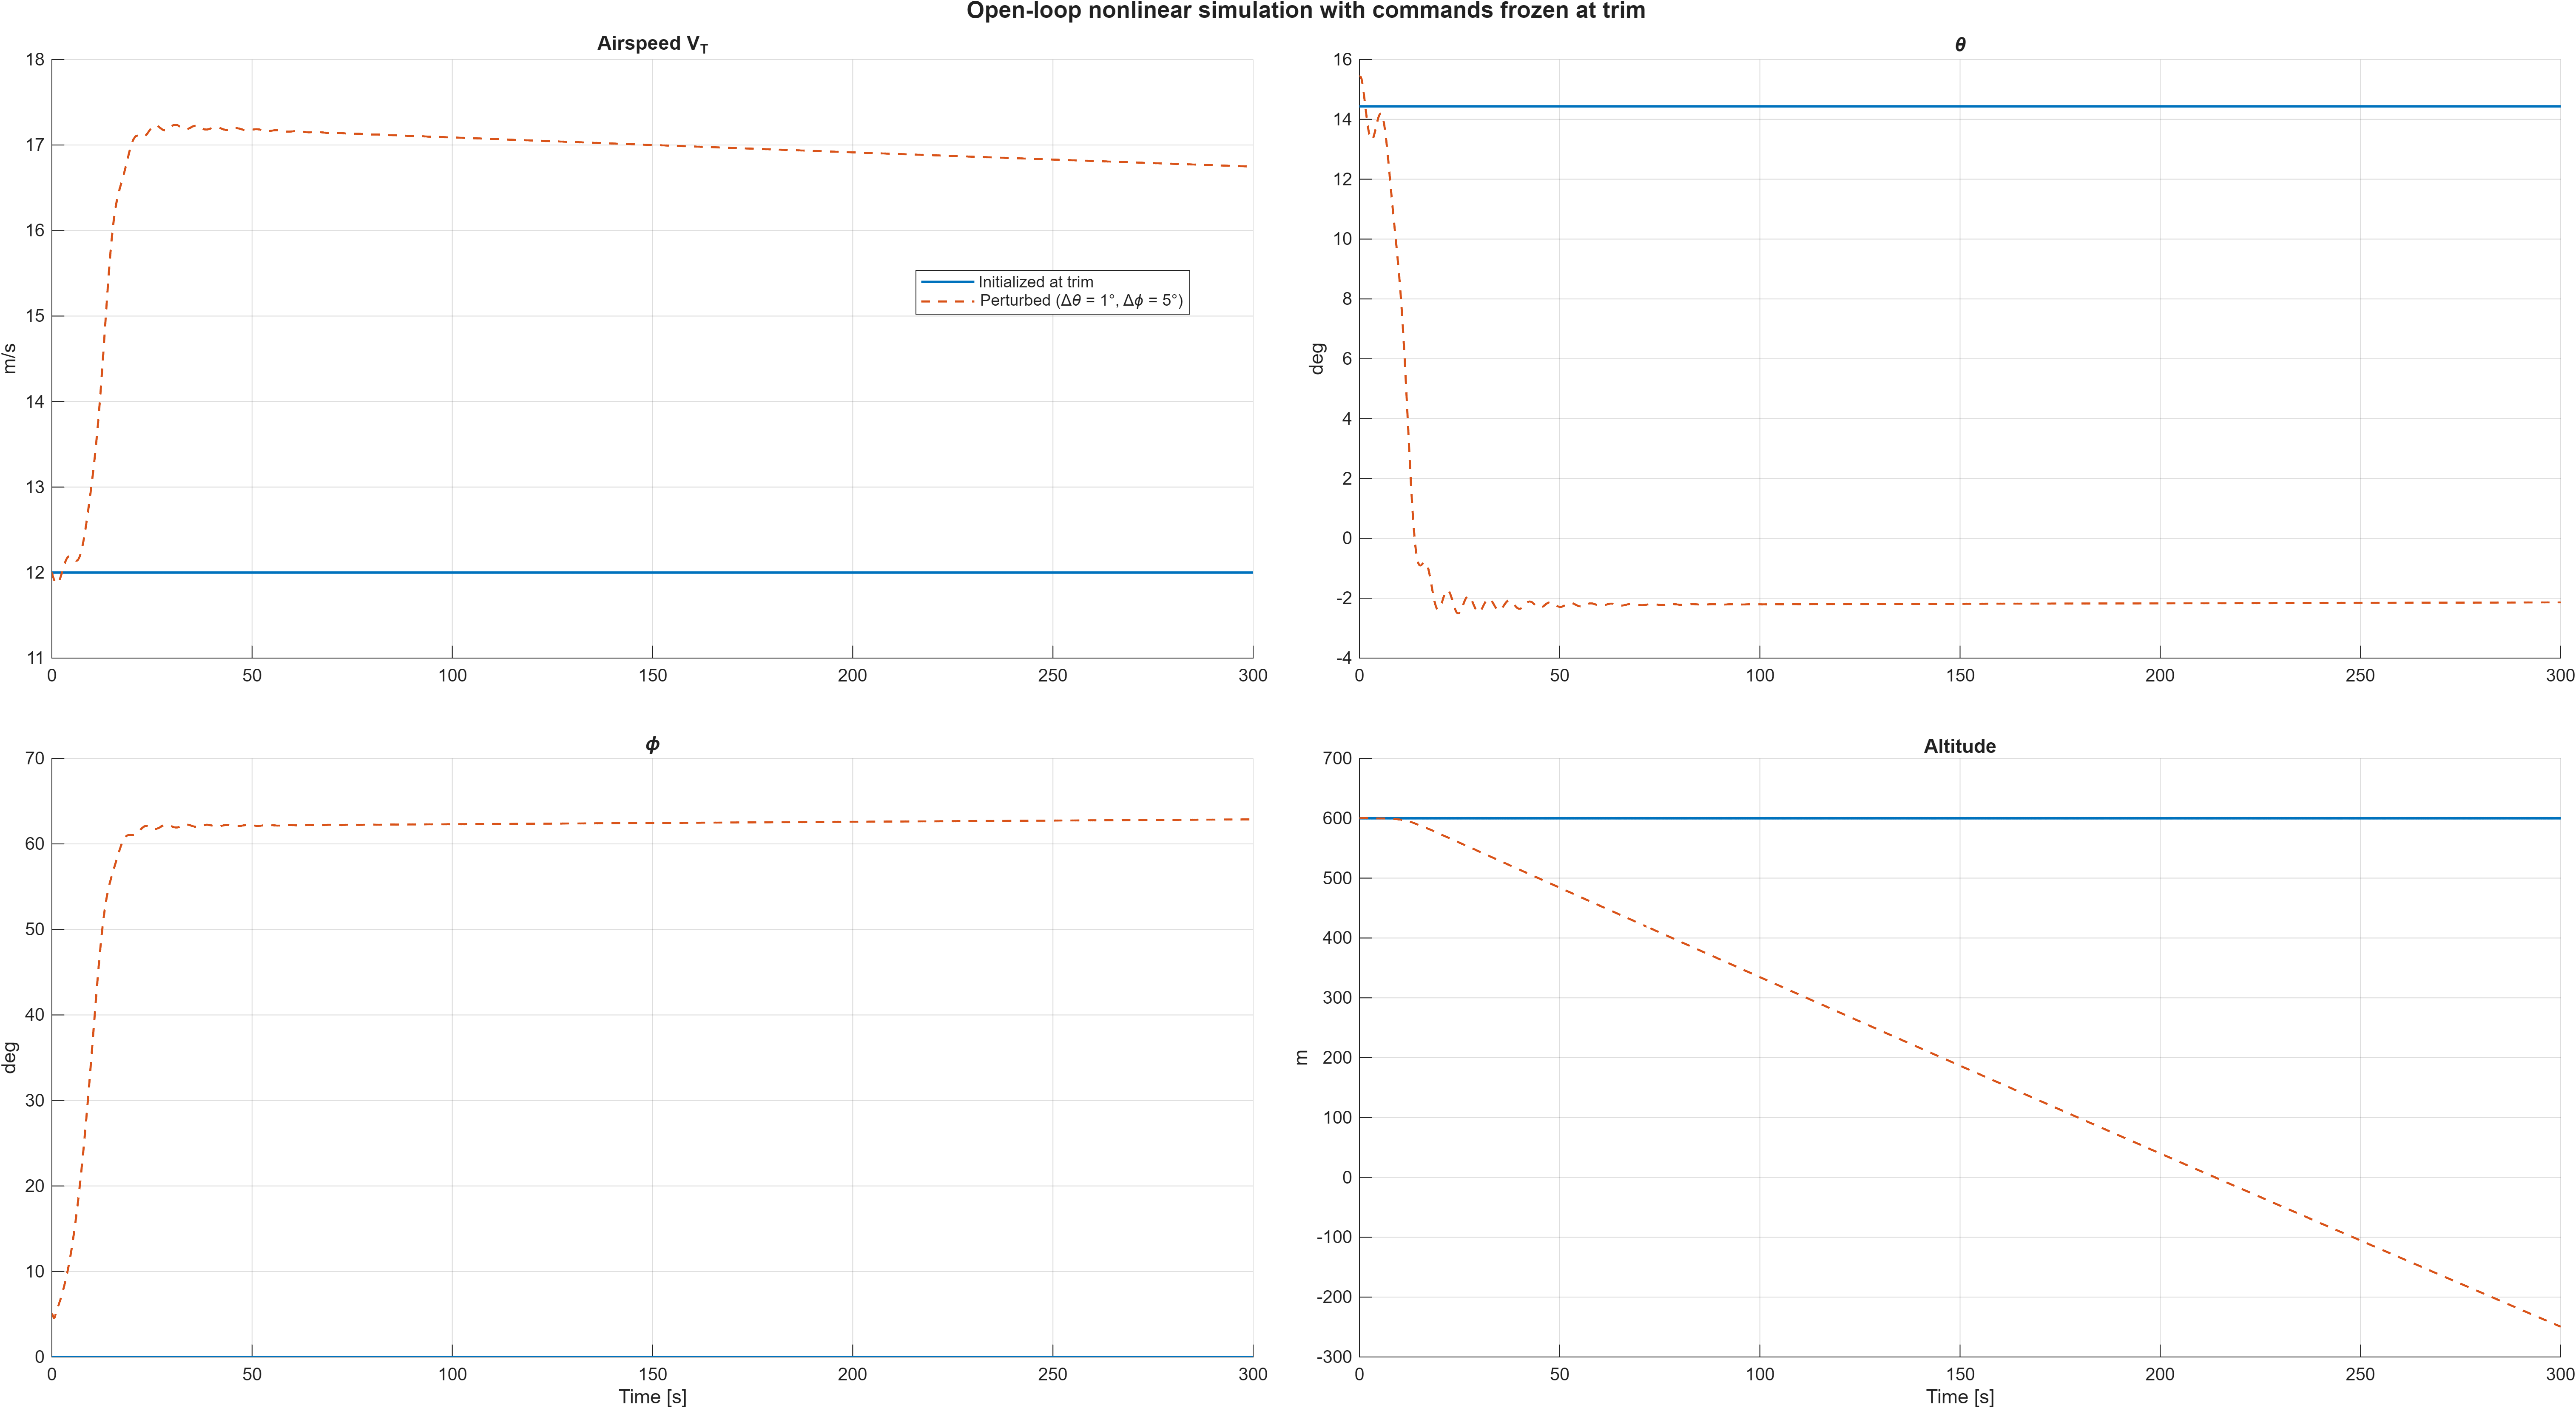
\includegraphics[width=\linewidth]{fig_malha_aberta.png}
\caption{Open-loop nonlinear simulation with commands frozen at trim.
Solid: initialized exactly at trim (remains at equilibrium). Dashed: small
initial perturbation --- the unstable spiral mode diverges.}
\label{fig:openloop}
\end{figure}

\section{Controller Design}
\label{sec:control}

\subsection{Closed-Loop Requirements}
\label{sec:requirements}
Both control laws are judged against the closed-loop requirements of
Table~\ref{tab:requirements}, adopted from the design practice of our
research group~\cite{mirko2026companion} and anchored, row by row, in
the flight-control literature. The stability-margin rows descend from the military
flight-control-system specification MIL-F-9490D, which requires a gain
margin of at least 6\,dB and a phase margin of at least $45^\circ$ for
the augmented airplane~\cite{milf9490d1975} --- limits carried into
present-day industry practice by its successor SAE
AS94900~\cite{sae2007as94900}; the 10\,dB adopted here is deliberately
conservative. The damping row is stricter than the flying-qualities
levels of MIL-F-8785C and MIL-STD-1797A, whose Level-1 bands admit
short-period and Dutch-roll damping well below
0.75~\cite{milf8785c1980,moorhouse1982milf8785c,milstd1797a1990}; the
$\zeta>0.75$ target reflects the classical well-damped second-order
response ($\zeta\approx0.7$ yields ${\approx}5\%$
overshoot~\cite{franklin2018feedback}). The time-domain rows
(settling time, overshoot, steady-state error) are outer-loop
performance targets in the sense of classical autopilot design
texts~\cite{blakelock1991automatic,nelson1998flight}, sized for this
platform's mission profile. Since these criteria were written for
piloted aircraft, their transfer to a small UAV is itself a design
decision, supported by the literature on scaled flying-qualities
requirements for unmanned aircraft~\cite{cotting2010evolution}.

\begin{table}[!t]
\caption{Closed-loop design requirements and their scope.}
\label{tab:requirements}
\centering
\begin{tabular}{lll}
\toprule
Requirement & Value & Scope \\
\midrule
Settling time & $<60$\,s & guidance channels ($\VT$, $\psi$, $h$) \\
Overshoot & $<10\%$ & guidance channels ($\VT$, $\psi$, $h$) \\
Steady-state error & $2$--$5\%$ & guidance channels ($\VT$, $\psi$, $h$) \\
Damping ratio & $\zeta>0.75$ & augmented inner modes \\
Gain margin & $>10$\,dB & each loop, at design \\
Phase margin & $>45^\circ$ & each loop, at design \\
\bottomrule
\end{tabular}
\end{table}

Each row carries an explicit scope. The time-domain rows apply to the
\emph{guidance-level} channels ($\VT$, $\psi$, $h$) on shaped
(prefiltered) mission references --- they are verified against both
controllers in Section~\ref{sec:sil-comparison}. The damping row
applies to the augmented inner modes at design time; the margin rows
are enforced per loop during loop shaping (the phase-margin targets of
Table~\ref{tab:gains}, $55$--$65^\circ$, exceed the requirement). One
honest caveat closes the picture: the augmented Dutch-roll damping
achieved by the PID design ($0.707$, Section~\ref{sec:pid}) satisfies
the MIL-F-8785C Level-1 band with wide margin but sits marginally
below the stricter internal target of $0.75$ --- reported as designed
rather than adjusted to fit. On the short-period side, the pitch-rate
damper gain of the tuning of record ($K_q=0.10$,
Section~\ref{sec:pid}) was raised precisely to lift the short-period
damping.

\subsection{Cascade PID Architecture}
\label{sec:pid}
The PID controller follows a classical cascade architecture ---
successive loop closure in the sense of~\cite{beard2012small} ---
designed loop by loop on the linearized models of
Section~\ref{sec:model} and then verified on the full nonlinear model.
The design methodology --- loop ordering, damper-first stability
augmentation, and the coordinated-turn heading law ---
follows~\cite{santos2018}, developed there for a conventional
general-aviation aircraft and applied here to the hybrid VTOL platform
in its fixed-wing flight mode.

\subsubsection{Stability Augmentation}
Rate dampers are closed first, tuned by root locus on the linear
subsystems. The pitch-rate damper $K_q\,q$ raises the short-period
damping ($K_q=0.10$ in the tuning of record, a deliberately raised
damping target); the yaw damper feeds $r$ through a washout
$s/(s+1)$ to the rudder, raising Dutch-roll damping to
$\zeta_{DR}\approx0.707$ without opposing steady turns. The washout
yaw damper is one of the oldest devices of automatic flight control:
introduced with the first swept-wing jets --- which could not be flown
unaugmented because of their Dutch roll --- in the late
1940s~\cite{mcruer1981eighty}, it received its definitive analytical
treatment in the classical stability-augmentation
literature~\cite{mcruer1973aircraft,blakelock1991automatic}, which the
present implementation follows. The roll
subsidence mode already meets Level~1 handling qualities with margin
($\lambda=-11.3$\,s$^{-1}$, Table~\ref{tab:poles}), so no roll-rate damper
is used ($K_p=0$).

\subsubsection{Longitudinal Loops}
\begin{itemize}
  \item \emph{Pitch-attitude inner loop} ($C_{\theta}$): PI on
        $\theta^{ref}-\theta$ to the elevator, closed over the $K_q$ damper;
  \item \emph{Airspeed hold} ($C_{vel}$): PI on $\VT^{ref}-\VT$ to the
        throttle;
  \item \emph{Altitude outer loop} ($C_{alt}$): PI on $h^{ref}-h$ to the
        pitch-attitude reference, with the command clamped to
        $\pm10^\circ$ and clamping-type anti-windup. The clamp is an
        angle-of-attack protection: with $\theta^{ref}$ limited to
        $+10^\circ$ about the trim, the peak $\alpha$ during an altitude
        capture stays near $16^\circ$ (the plant model has no stall
        representation, so the limit is imposed by design).
\end{itemize}
Depending on the flight mode, the pilot-level selector engages either the
altitude cascade (\emph{AltitudeHold}) or direct pitch tracking
(\emph{ThetaHold}), in which case the altitude loop is open.

\subsubsection{Lateral--Directional Loops}
\begin{itemize}
  \item \emph{Bank inner loop} ($C_{\phi}$): PI on $\phi^{ref}-\phi$ to
        the aileron (negative gains, since $C_{l_{\delta_a}}<0$);
  \item \emph{Heading hold} ($K_{heading}$): proportional law
        $\phi^{ref}=K_{heading}(\psi^{ref}-\psi)$ with
        $K_{heading}=u^e/(g\,\tau_\psi)$ and $\tau_\psi=6$\,s, the
        coordinated-turn relation~\cite{santos2018}. As with the
        longitudinal channel, the mode selector engages either heading
        hold (\emph{PsiHold}) or direct bank commands (\emph{PhiHold}).
\end{itemize}

\subsubsection{Tuning and Resulting Gains}
The compensators are PI ($K_d=0$): damping is provided by the explicit
dampers rather than by derivative action, which also avoids differentiating
noisy rate measurements on the embedded target. Each loop was tuned by
loop shaping (\texttt{pidtune}) with \emph{sequential inner-first} closure
--- every outer loop is designed against the already-closed inner
dynamics --- targeting the crossover frequencies and margins listed in
Table~\ref{tab:gains}, with a bandwidth separation of 5--7$\times$ between
consecutive loops.

\begin{table}[!t]
\caption{PID loops: design targets and resulting gains (tuning of
record).}
\label{tab:gains}
\centering
\begin{tabular}{llccl}
\toprule
Loop & Map & $K_P$ & $K_I$ & Original target \\
\midrule
$C_\theta$ & $\theta^{ref}\!\to\!\delta_e$ & 0.917 & 0.857 & $\omega_c$=2.0, PM=65$^\circ$ \\
$C_{vel}$ & $\VT^{ref}\!\to\!\delta_t$ & 0.32 & 0.096 & $\omega_c$=0.8 \\
$C_{alt}$ & $h^{ref}\!\to\!\theta^{ref}$ & 0.050 & 0.0043 & $\omega_c$=0.35, PM=55$^\circ$ \\
$C_\phi$ & $\phi^{ref}\!\to\!\delta_a$ & $-0.45$ & $-0.036$ & $\omega_c$=2.0, PM=65$^\circ$ \\
$K_{heading}$ & $\psi^{ref}\!\to\!\phi^{ref}$ & 0.1975 & --- & $\tau_\psi$=6\,s \\
$K_q$ & $q\!\to\!\delta_e$ & 0.10 & --- & $\zeta_{SP}$ raised \\
$K_r$ & $r\!\to\!\delta_r$ (washout) & 0.1481 & --- & $\zeta_{DR}$=0.707 \\
\bottomrule
\end{tabular}
\end{table}

The outer altitude and airspeed loops use two-degree-of-freedom
setpoint weighting with $b=0$ --- the proportional term acts on the
measured output only, with the reference entering through the integral
path --- and this tuning of record, retuned against the requirements
of Table~\ref{tab:requirements}, is the configuration used in every
campaign of this article, matching the public repository HEAD.

A command prefilter $1/(\tau_{ref}s+1)$ with $\tau_{ref}=3$\,s is applied
to the \emph{increment} of each reference before the loops, giving a
two-degree-of-freedom structure in the tradition of reference command
shaping~\cite{singer1990preshaping}: the command response is smoothed
--- the raw step would otherwise demand an unrealizable actuator jump
--- without altering the feedback design, its margins, or the clamp. This detail
matters for the embedded deployment: in the HIL architecture of
Section~\ref{sec:hil} the references travel through the link
\emph{already filtered}, so the prefilter stays on the host and only the
feedback path is embedded.

With all loops closed, the linear closed-loop system is stable with every
pole in the left half-plane: the slowest mode is at $-0.127$\,s$^{-1}$ and
the minimum damping ratio among the oscillatory modes is $\zeta=0.55$.
Notably, the open-loop unstable spiral mode ($+0.233$\,s$^{-1}$,
Table~\ref{tab:poles}) is stabilized at $-0.143$\,s$^{-1}$.

\subsection{Output-Feedback LQR (LQRy)}
\label{sec:lqry}
The second control law is a linear--quadratic design with \emph{output}
weighting (LQRy): for each loop, the quadratic cost
\begin{equation}
J=\int_0^\infty\!\big(y^{\!\top}Q\,y+u^{\!\top}R\,u\big)\,dt,\qquad y=C_{syn}x,
\end{equation}
is minimized over the linearized models of Section~\ref{sec:model},
yielding constant gains on the measured states plus integral action on
the tracked error. This is the classical linear--quadratic regulator
of Kwakernaak and Sivan~\cite{kwakernaak1972linear} in the
constant-gain \emph{output-feedback} setting introduced by Levine and
Athans~\cite{levine1970output} --- a problem whose difficulty and
solution landscape are surveyed in~\cite{syrmos1997static}, and whose
standard numerical solution is the flight-control-motivated iterative
algorithm of Moerder and Calise~\cite{moerder1985convergence}; the
formulation and its application to aircraft control follow the
treatment of Stevens \emph{et al.}~\cite{stevens2016aircraft}. The
weight-selection rationale follows established LQ design
practice~\cite{anderson1990optimal}, starting from Bryson's
rule~\cite{bryson1975applied}. The design compared in this article is
the \emph{gain-scheduled} LQRy of the companion article by the second
author~\cite{mirko2026companion}, which details its synthesis ---
including the target-transmission-zero augmentation and the gain
scheduling over the flight envelope --- and its frequency-domain
(Nichols) robustness assessment; it is summarized here.

The architecture deliberately mirrors the PID mode structure, so that
the two laws face the same tasks: five independent designs ---
\emph{ThetaHold}, \emph{AltitudeHold} (cascading into
$\theta^{ref}$), \emph{VelHold}, \emph{PhiHold} (a $2\times2$ design
commanding aileron and rudder), and \emph{PsiHold} (cascading into
$\phi^{ref}$) --- selected by the same three mode switches used by the
PID (Table~\ref{tab:lqry-loops}). Each synthesis model augments the
relevant linear subsystem with a frequency-selective filter
\begin{equation}
G(s)=\frac{s^{2}+2\zeta\omega_{n}s+\omega_{n}^{2}}{s}
\end{equation}
on each tracked output --- imposing target transmission zeros that
shape the closed loop while providing the integral action --- plus a
first-order actuator lag at 24\,rad/s; the constant output-feedback
gains are obtained from the coupled Lyapunov equations of the LQ
output-feedback problem~\cite{levine1970output,moerder1985convergence}.
The design is synthesized at nine envelope conditions
(12/15/18\,m/s $\times$ 590/600/610\,m); the SIL comparison of
Section~\ref{sec:sil} exercises the condition-2 (12\,m/s, 600\,m) gain
set, consistent with the mission's initial trim --- mid-mission gain
switching is not exercised. The weights per condition are given in the
companion article~\cite{mirko2026companion}.

\begin{table}[!t]
\caption{LQRy loops: regulated output and actuator (weights per
envelope condition in the companion article~\cite{mirko2026companion}).}
\label{tab:lqry-loops}
\centering
\begin{tabular}{lll}
\toprule
Loop & Output & Actuator \\
\midrule
ThetaHold & $\theta$ & elevator \\
AltitudeHold & $h\!\to\!\theta^{ref}$ & elevator \\
VelHold & $\VT$ & throttle \\
PhiHold & $\phi$, $\beta$ & ail.+rud. \\
PsiHold & $\psi\!\to\!\phi^{ref}$ & aileron \\
\bottomrule
\end{tabular}
\end{table}

Table~\ref{tab:lqry-gains} records the condition-2 gains: these are
the values used in the SIL comparison of Section~\ref{sec:sil}. Two
structural remarks: the pitch design feeds back the elevator
(actuator) state itself, its synthesis model carrying the 24\,rad/s
lag as a fifth state; and the $2\times2$ lateral design carries a
sideslip-integral gain alongside the bank integral (0.00845 on the
aileron and 0.02023 on the rudder at condition~2) --- small relative
to the $\phi$ integral, but not negligible. The earlier
\emph{fixed-gain} LQRy delivery, deployed on the HIL bench of
Section~\ref{sec:hil}, used a different, softer gain set, available in
the repository~\cite{repo}.

\begin{table}[!t]
\caption{LQRy gains at envelope condition 2 (12\,m/s, 600\,m), as used
in the SIL comparison (4 significant digits). Convention:
$u=G_{x}\,x+K_{I}\!\int\!e\,dt$. The $K_I$ column of PhiHold is the
bank ($\phi$) integral gain.}
\label{tab:lqry-gains}
\centering
\resizebox{\linewidth}{!}{%
\begin{tabular}{llll}
\toprule
Loop & State vector $x$ & $G_{x}$ & $K_I$ \\
\midrule
ThetaHold & $[\VT\,\alpha\,q\,\theta\,\delta_e]$ &
$[-0.00461\;6.477\;-15.60\;-483.2\;-6.795]$ & $-625$ \\
AltitudeHold & $[\VT\,\alpha\,q\,\theta\,h]$ &
$[-0.0718\;4.474\;-0.2121\;-5.064\;-0.5086]$ & $-0.2025$ \\
VelHold & $[\VT\,\alpha\,q\,\theta]$ &
$[-78.81\;-0.9055\;0.0589\;1.306]$ & $-50$ \\
PhiHold (ail.) & $[\beta\,p\,r\,\phi]$ &
$[0.00693\;0.01013\;0.03505\;0.1595]$ & $0.1720$ \\
PhiHold (rud.) & $[\beta\,p\,r\,\phi]$ &
$[-0.01085\;-0.02236\;-0.08167\;-0.3542]$ & $-0.3595$ \\
PsiHold & $[\beta\,p\,r\,\phi\,\psi]$ &
$[-5.387\;-0.1123\;-0.7948\;-1.272\;-6.037]$ & $-7.773$ \\
\bottomrule
\end{tabular}}
\end{table}

Unlike the PID harness, the LQRy harness of the gain-scheduled design
includes first-order actuator lags (24\,rad/s on the surfaces, 0.1\,s
on the throttle) and a $[0,1]$ throttle saturation, but no rate
limits, no surface position saturations, no reference prefilter, and
no $\theta^{ref}$ clamp --- references enter the loops as raw steps.
These differences between the two design harnesses are consolidated
and discussed in Section~\ref{sec:protocol}.

\subsection{Roll-to-Longitudinal Coupling}
\label{sec:coupling}
Both designs treat the longitudinal and lateral--directional channels
independently, so the classical roll-to-pitch coupling --- banking
tilts the lift vector, and the lift deficit, proportional to
$1-\cos\phi$, drops the nose and costs altitude --- is handled by
feedback alone. Since this is a deliberate design choice, it was
quantified rather than assumed benign: both controllers --- the PID
tuning of record and the gain-scheduled LQRy --- were subjected
to bank captures of increasing amplitude ($\phi^{ref}$ steps of
$5/15/30^\circ$ at $t=20$\,s, each rig shaping the reference as its
harness prescribes), in \emph{ThetaHold} (altitude loop open, the
worst case) and in \emph{AltitudeHold}, with all longitudinal metrics
taken as deviations from each rig's own $\phi=0$ baseline
(Fig.~\ref{fig:coupling}).
\begin{figure}[!t]\centering
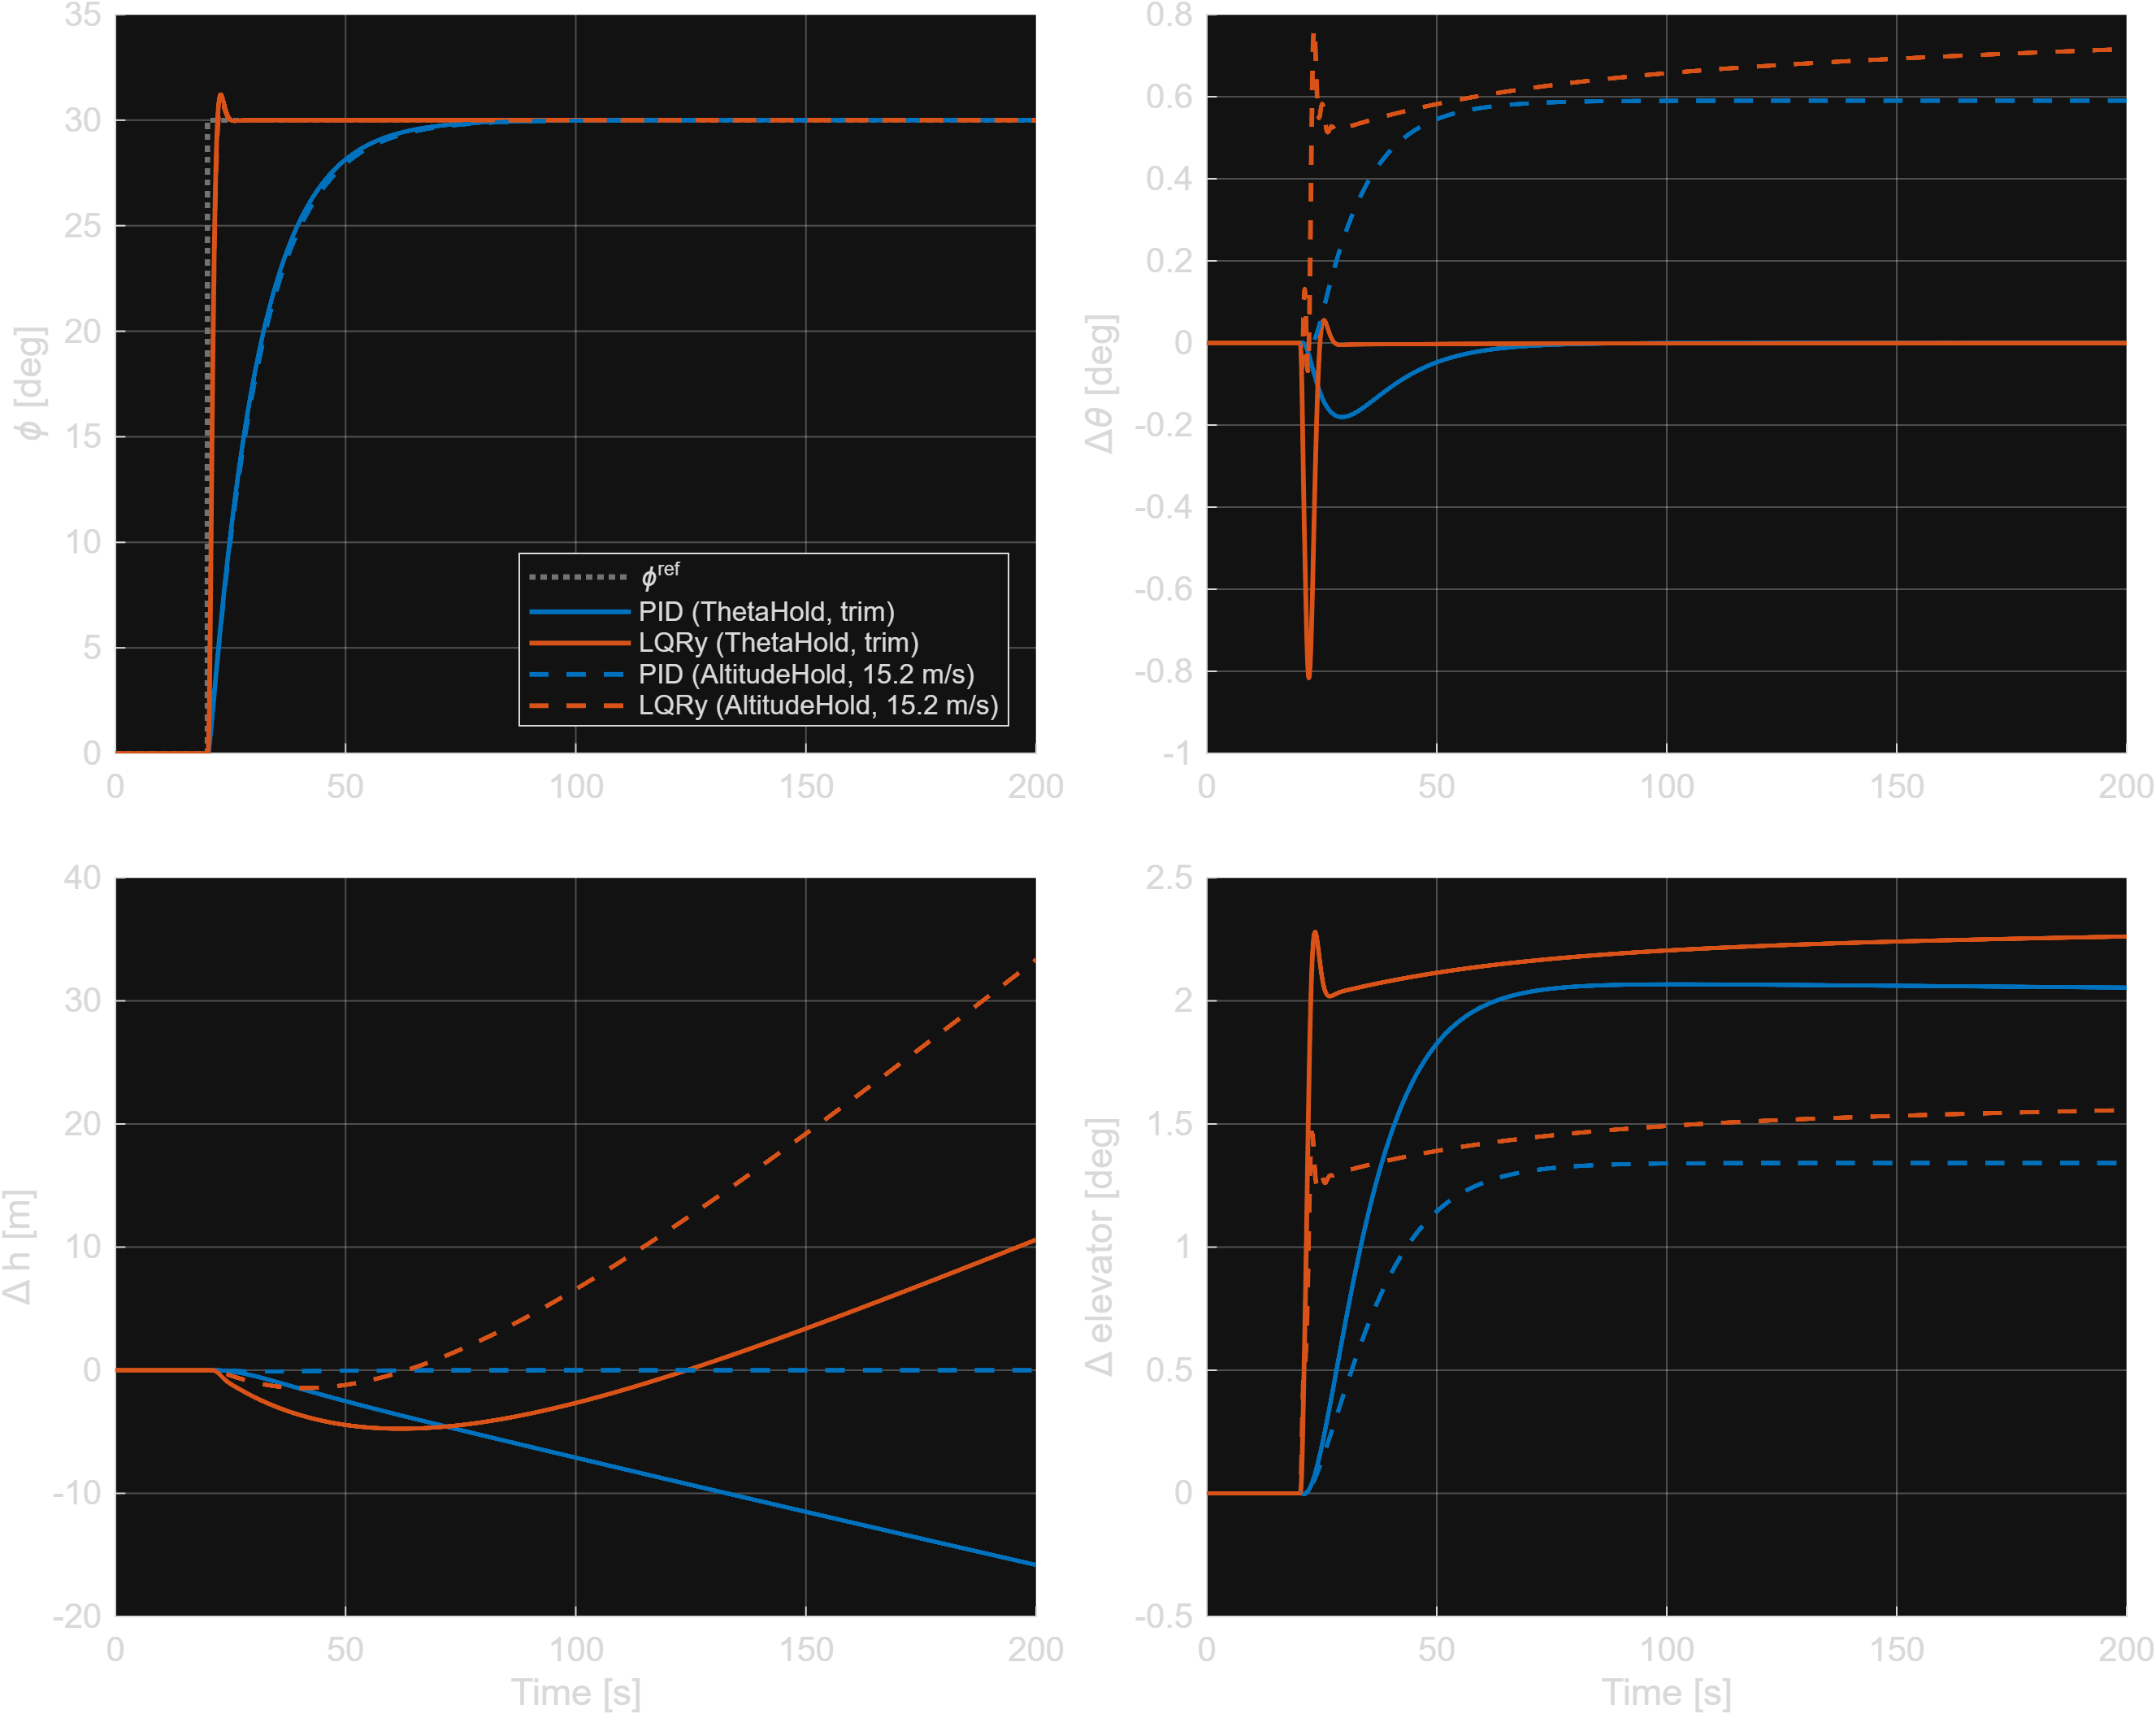
\includegraphics[width=\linewidth]{fig_acoplamento.png}
\caption{Roll-to-longitudinal coupling, $\phi^{ref}=30^\circ$ step at
$t=20$\,s: $\phi$ (with the reference), $\Delta\theta$,
$\Delta h$, and $\Delta$elevator relative to each configuration's
$\phi=0$ baseline. Solid: ThetaHold at the 12\,m/s trim; dashed:
AltitudeHold at 15.2\,m/s.}\label{fig:coupling}\end{figure}

The results confirm the mechanism and bound its size. For the PID in
ThetaHold, the transient pitch dip scales with $1-\cos\phi$ as
expected --- $-0.005^\circ$, $-0.04^\circ$, and $-0.18^\circ$ for
$5/15/30^\circ$ --- negligible at the $5^\circ$ amplitude of the
flight campaign. The LQRy dip is $4$--$5\times$ larger
(${\approx}-0.8^\circ$ at $30^\circ$): its multivariable structure
does \emph{not} natively absorb the coupling better than the cascade.
With the altitude loop open the altitude drifts by construction ---
$-15.8$\,m for the PID over 200\,s at $30^\circ$, while the LQRy,
whose high-bandwidth airspeed loop adds energy through the turn,
drifts $+10.6$\,m \emph{upward}; closing
the altitude loop absorbs the coupling, with $\theta^{ref}$ settling
higher ($+0.59^\circ$ PID, $+0.71^\circ$ LQRy) and $\Delta h$
returning to zero after a transient dip of $0.10$\,m (PID) and
$1.45$\,m (LQRy), at the cost of a small steady
elevator increment.

In the steady turn, the elevator increment is \emph{larger} in the
ThetaHold runs at the 12\,m/s trim (solid traces, $2.06^\circ$ PID
and $2.26^\circ$ LQRy) than in the AltitudeHold runs at 15.2\,m/s
(dashed, $1.34^\circ$ and $1.55^\circ$), which at first seems
backwards ---
why would the altitude-holding configuration need \emph{less}
elevator? The explanation is the operating point, not the mode: sustaining the same $30^\circ$ bank
(load factor $1/\cos 30^\circ = 1.15$) requires an increment of lift
that, at 15.2\,m/s, is produced with less angle of attack --- and less
elevator --- because the dynamic pressure is $(15.2/12)^2 = 1.6$ times
higher. The measured increment ratios ($0.65$ for the PID, $0.69$ for
the LQRy) sit within a few
percent of the dynamic-pressure prediction $(12/15.2)^2 = 0.62$, the
residual owing to the $\theta^{ref}$ adjustment and the
angle-of-attack dependence of drag.

In answer to the natural question --- no, no feedforward decoupling
term is used by either law ($K_{f\!f}=0$ throughout): with the
altitude loop closed the residual coupling is $0.10$\,m even at a
$30^\circ$ bank (PID), and at the $5^\circ$ amplitude of the flight
campaign the $1-\cos\phi$ factor is a further $35\times$ smaller, so
feedback suffices.
A feedforward stage, and its evaluation on both laws at larger bank
angles, is left as future work
(Section~\ref{sec:conclusion}).

\section{Closed-Loop Simulations (SIL)}
\label{sec:sil}

\subsection{Remark on Trim Commands}
\label{sec:sil-trim}
% Nota pedida pela orientadora: deixar clara a questao do delta-comando de
% trimagem vs deltas dados nas simulacoes.
All controllers in this work operate on \emph{incremental} commands about
the trim condition of Section~\ref{sec:trim}: the compensators output
$\Delta\delta$, and the trim commands $\delta^e$
of~\eqref{eq:dtrim} are added before the actuator models. Consequently,
whenever a simulation reports a command signal, the reader should
distinguish the absolute command $\delta = \delta^e + \Delta\delta$ from
the increment $\Delta\delta$ produced by the controller. In steady flight
at the trim point, the absolute commands settle at $\delta^e$ (e.g., the
elevator at $7.62^\circ$), not at zero.

\subsection{Comparison Protocol and Known Asymmetries}
\label{sec:protocol}
Every head-to-head result in this article follows the same protocol
--- in the spirit of the experimental controller benchmarks of the
recent literature~\cite{okasha2022design,rinaldi2023comparative}: the
\emph{same} nonlinear plant, the \emph{same} reference amplitudes
and timings, and the \emph{same} metric windows, with each control law
running in its own design harness, exactly as delivered. That last
clause matters, because the two harnesses are not identical, and an
honest comparison must say so. Three asymmetries are known and
uncontrolled:
\begin{enumerate}
  \item \emph{Actuator models.} The PID harness includes the full
        actuator chain of Section~\ref{sec:model} (position and rate
        saturations, first-order servo and engine lags). The LQRy
        harness includes first-order actuator lags --- 24\,rad/s on
        the surfaces versus the 20\,rad/s assumed on the PID side,
        and 0.1\,s versus 0.30\,s for the throttle --- and a $[0,1]$
        throttle saturation, but omits the rate limits and surface
        position saturations of the PID harness.
  \item \emph{Reference shaping.} The PID applies the
        $1/(3s+1)$ prefilter of Section~\ref{sec:pid} to every
        reference increment; the LQRy receives raw reference steps.
  \item \emph{Protection logic.} The $\pm10^\circ$ $\theta^{ref}$
        clamp and its anti-windup exist only in the PID cascade.
\end{enumerate}

To bound the effect of these asymmetries on the conclusions, the PID
scenarios were repeated in an \emph{equalized} configuration ---
actuator bandwidth matched to 24\,rad/s, rate limits removed, clamp
and prefilter disabled, matching the LQRy harness.
Fig.~\ref{fig:eq-comb} overlays the two PID configurations on the
combined scenario: the equalization shifts the guidance captures
moderately --- airspeed rise time from 9.5 to 5.8\,s and settling from
18.0 to 11.4\,s, heading settling from 33.0 to 29.3\,s, altitude
settling from 44.4 to 40.8\,s, all with zero overshoot --- without
changing any comparative conclusion drawn below.

\begin{figure}[!t]
\centering
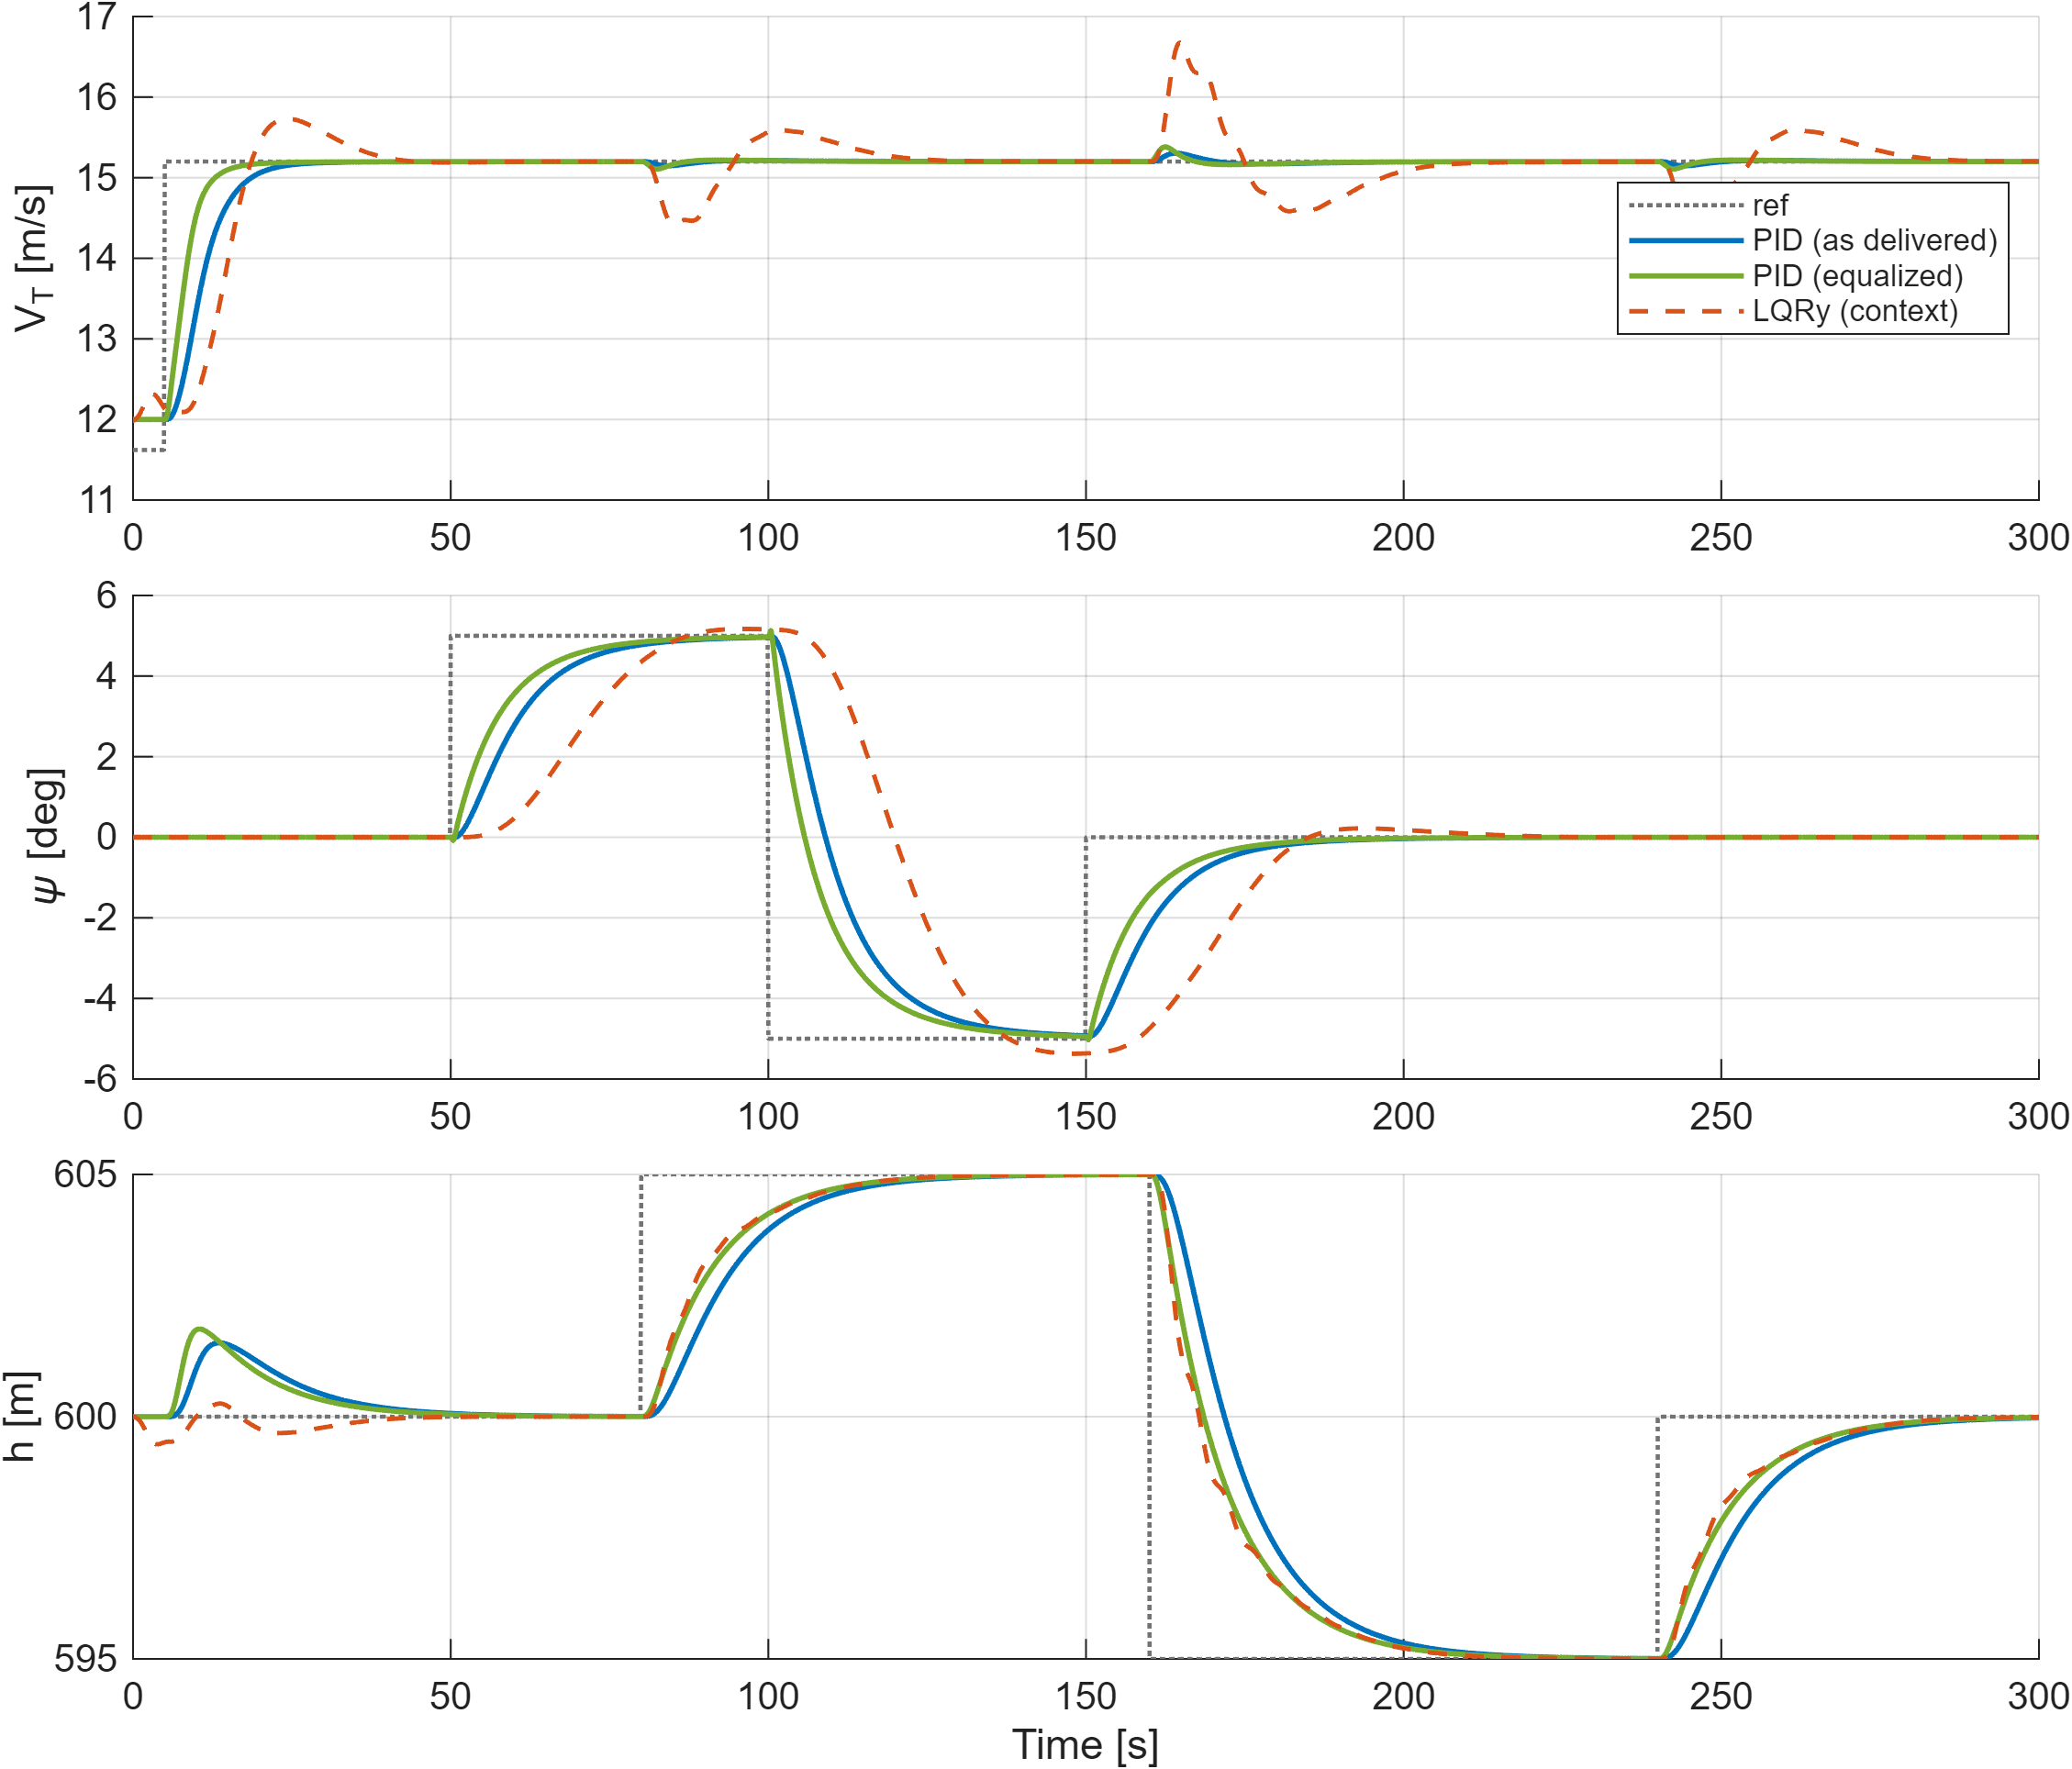
\includegraphics[width=\linewidth]{fig_eq_comb.png}
\caption{Equalization ablation, combined scenario: PID as delivered
vs.\ PID with the harness equalized to the LQRy rig (24\,rad/s
actuators, no rate limits, no clamp, no prefilter), with the LQRy
response for context.}
\label{fig:eq-comb}
\end{figure}

Two further implementation notes complete the disclosure. First, an
earlier fixed-gain LQRy build fed back the \emph{absolute} state
instead of the deviation from trim, producing a start-up kick (initial
elevator command of $4.11^\circ$ instead of the trim $7.62^\circ$);
the gain-scheduled build compared here feeds back trim deviations by
construction, and its runs were verified to start at the trim command.
The embedded (incremental-form) implementation of
Section~\ref{sec:hil} was immune to this distinction throughout.
Second, the LQRy rig initializes the plant at $\VT=12.0$\,m/s while
its stored controller trim corresponds to 11.62\,m/s, so LQRy runs
begin with a small longitudinal offset that the airspeed loop resolves
before the first reference event.

\subsection{PID on the Nonlinear Model}
\label{sec:sil-pid}
The cascade PID was evaluated on the nonlinear model under three
maneuvers, with the linear closed-loop response overlaid in each case:
a longitudinal climb ($h$ $+10$\,m), a lateral--directional heading change
($\psi$ $+15^\circ$), and an aggressive combined maneuver ($h$ $+30$\,m and
$\psi$ $+40^\circ$ commanded simultaneously, saturating the
$\theta^{ref}$ clamp for ${\approx}10$\,s).
Fig.~\ref{fig:nl-lin} shows the combined case. Linear and nonlinear
responses agree closely even in the aggressive maneuver (maximum
deviations of 0.38\,m in altitude, $0.52^\circ$ in pitch, and
$0.27^\circ$ in bank; below 0.21\,m/$0.75^\circ$/$0.05^\circ$ in the
single-axis maneuvers), validating both the linearization and the
linear-design--nonlinear-verification workflow. This validation was
performed with the original loop-shaping tuning; its conclusion ---
the fidelity of the linearization --- is independent of the
subsequent requirements-driven retune.

\begin{figure}[!t]
\centering
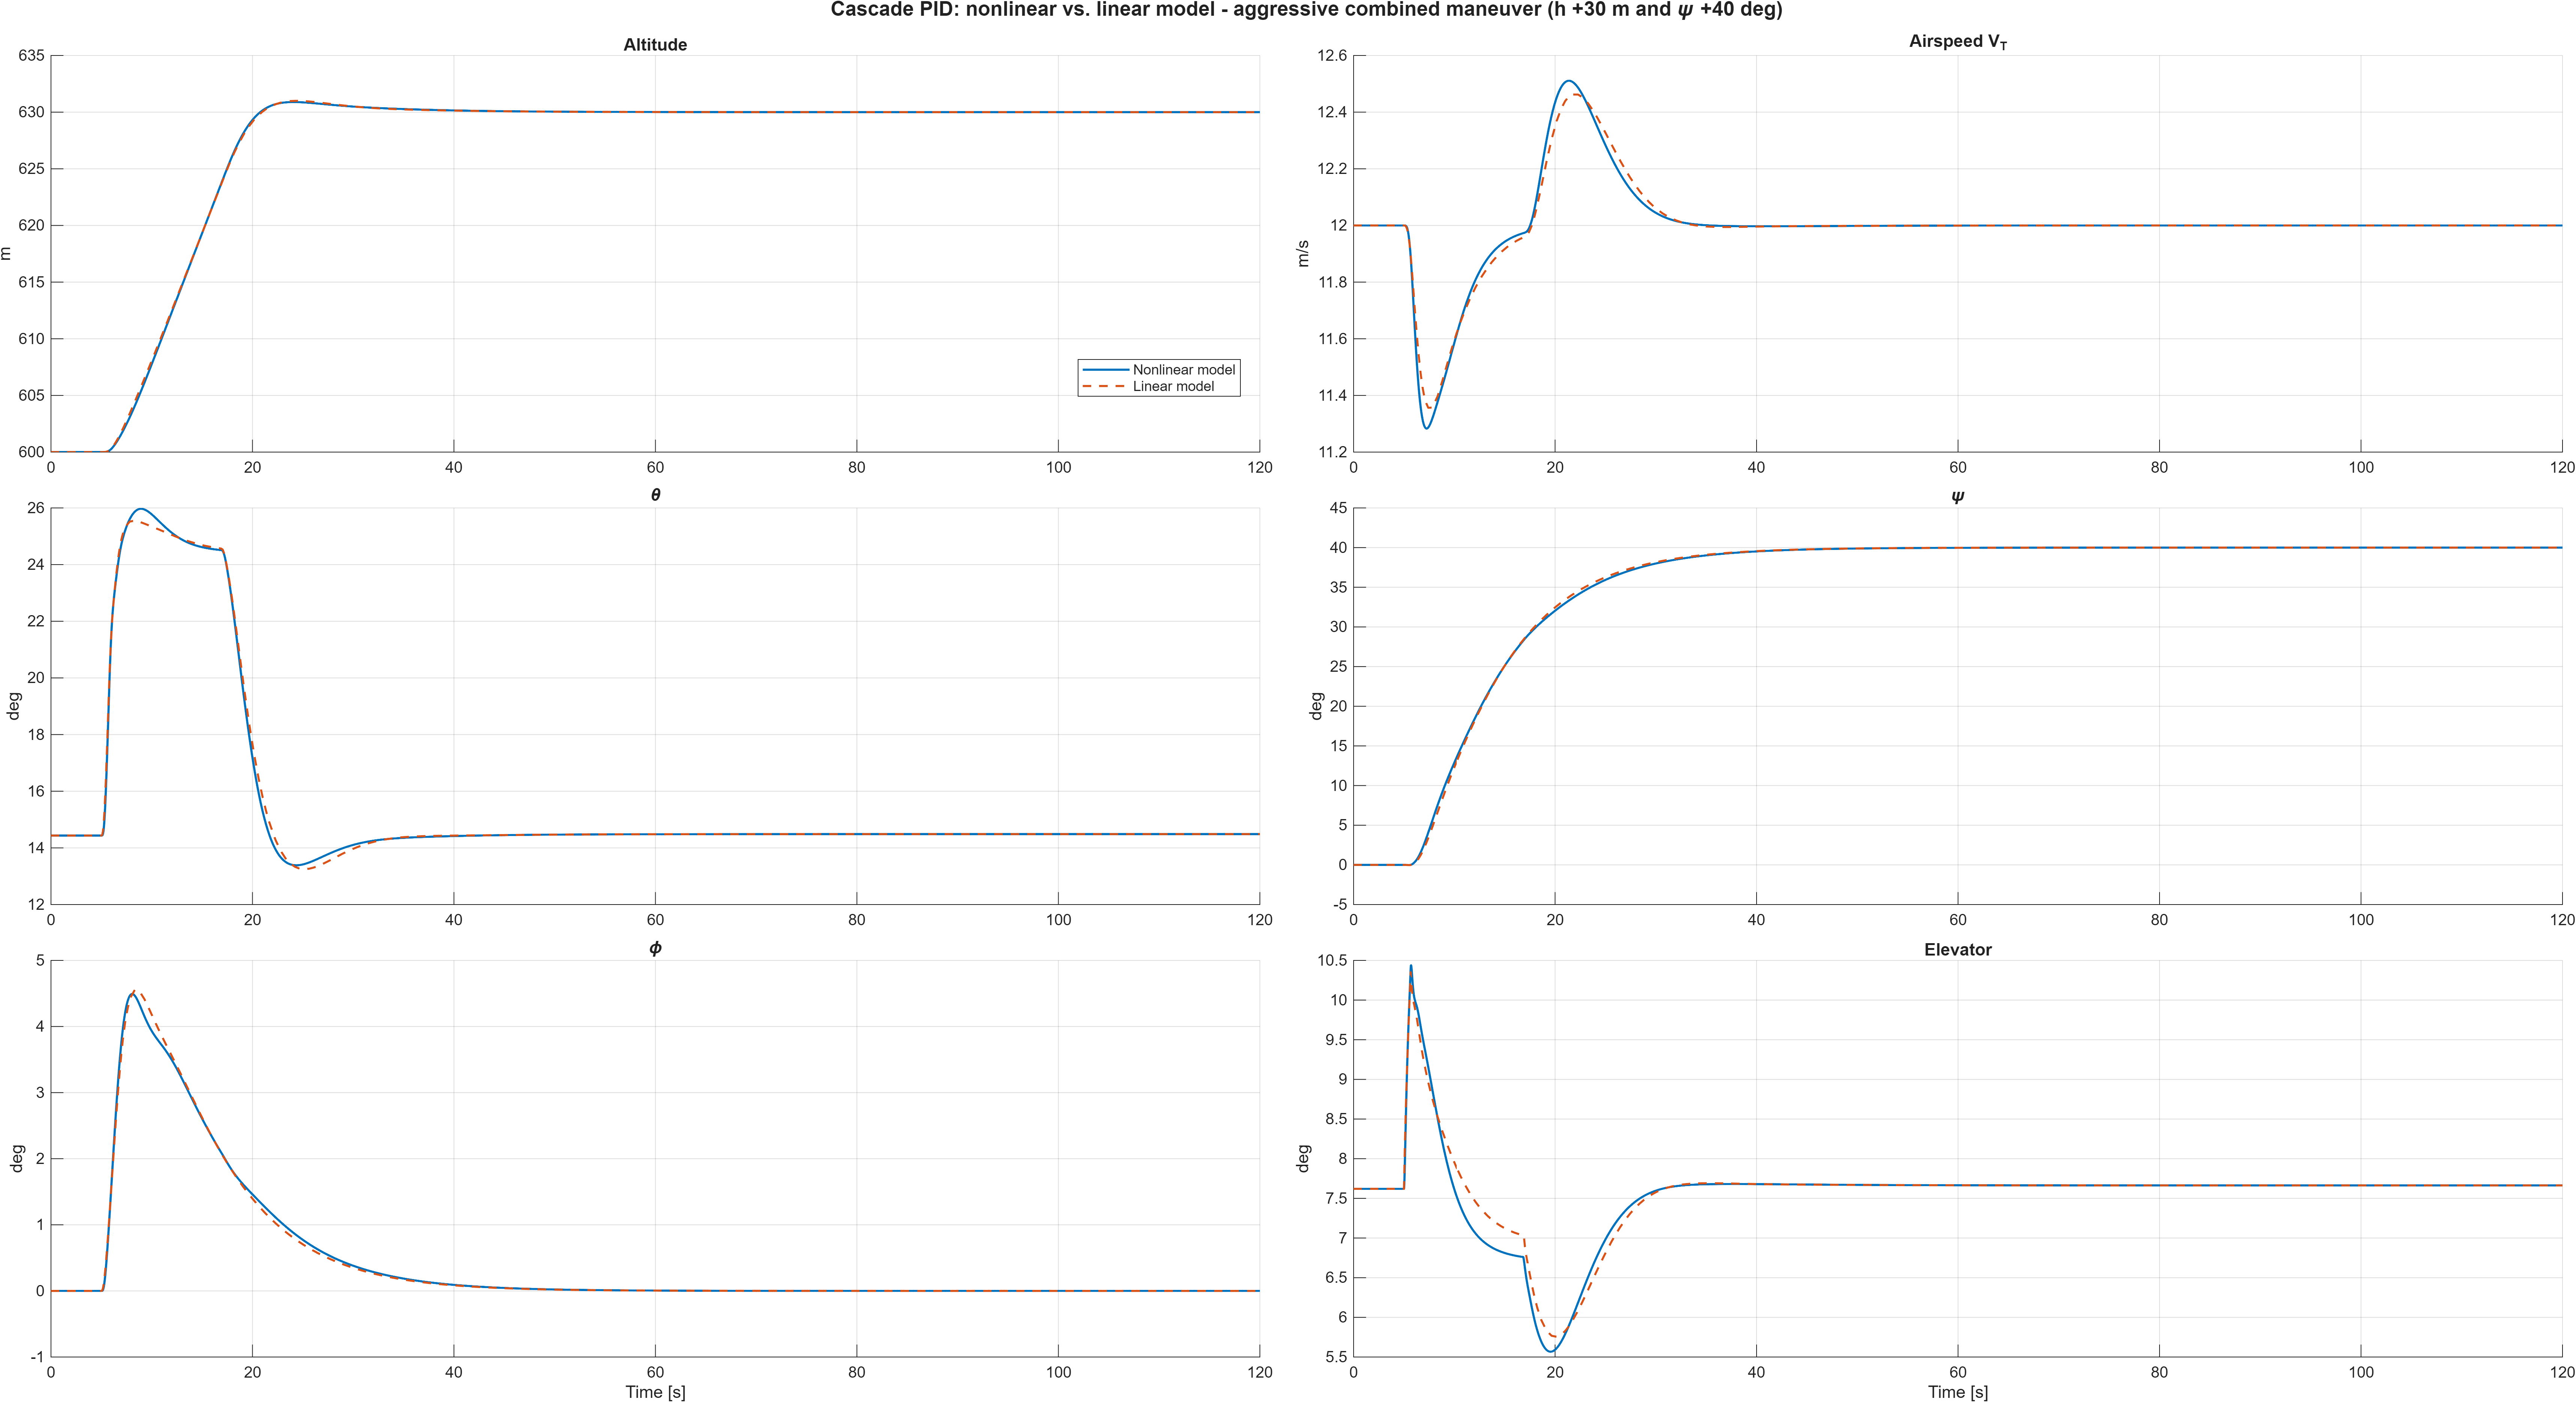
\includegraphics[width=\linewidth]{fig_nl_lin_agressiva.png}
\caption{PID, aggressive combined maneuver ($h$ $+30$\,m and $\psi$
$+40^\circ$ simultaneous): nonlinear model vs.\ linear closed loop.}
\label{fig:nl-lin}
\end{figure}

\subsection{LQRy on the Nonlinear Model}
\label{sec:sil-lqry}
The LQRy was evaluated directly on the nonlinear model, in its own
harness, under the same maneuver set used for the comparison below.
Its closed-loop character is consistent across maneuvers: fast,
high-bandwidth captures --- airspeed and altitude in ${\approx}6$\,s
with essentially no overshoot, heading in ${\approx}13$\,s with
visible overshoot (Table~\ref{tab:metrics}). Unlike the PID case, no linear-overlay
validation is presented: the linear design models of
Section~\ref{sec:lqry} are the basis of the synthesis, and the
nonlinear evaluation here is the verification step of record for the
delivered design.

\subsection{Controller Comparison}
\label{sec:sil-comparison}
The evaluation maneuvers deserve a word of justification. Doublets are
the conventional, well-characterized excitation of flight-test
practice --- originally for identification, where their frequency
content is matched to the modes of
interest~\cite{morelli1999flight,klein2006aircraft} --- and step and
doublet captures underlie the demonstration requirements of the
flying-qualities specifications~\cite{milf8785c1980}. For
\emph{unmanned} aircraft, however, the literature argues that
mission-based evaluation is the most transferable criterion, since
manned handling-qualities metrics do not carry over
directly~\cite{greene2014toward}; command-profile tracking of
airspeed, altitude, and attitude remains the standard validation
practice for small-UAV control laws~\cite{shen2025model}. The
campaign therefore uses both: per-axis guidance scenarios to
characterize each channel, and a 300\,s \emph{combined mission}
(airspeed step, heading doublet, altitude doublet, overlapping in
time) as the mission-level verdict.

The two controllers are compared on the nonlinear model under four
guidance-level scenarios
(\emph{VelHold}+\emph{PsiHold}+\emph{AltitudeHold}) with
\emph{identical} reference profiles on both rigs (amplitudes injected
into each rig's unmodified reference harness):
\begin{enumerate}
  \item \emph{Airspeed}: step $12\!\to\!15.2$\,m/s at 5\,s;
  \item \emph{Heading}: doublet of $\pm5^\circ$ at 50/100/150\,s;
  \item \emph{Altitude}: doublet of $\pm5$\,m at 80/160/240\,s;
  \item \emph{Combined mission}: all three simultaneously, 300\,s
        (flight case~4 of the campaign of Section~\ref{sec:hil}).
\end{enumerate}
Table~\ref{tab:metrics} reports the classical step-response metrics
per guidance channel, and Fig.~\ref{fig:cen-comb} shows the
combined mission.
\begin{figure}[!t]\centering
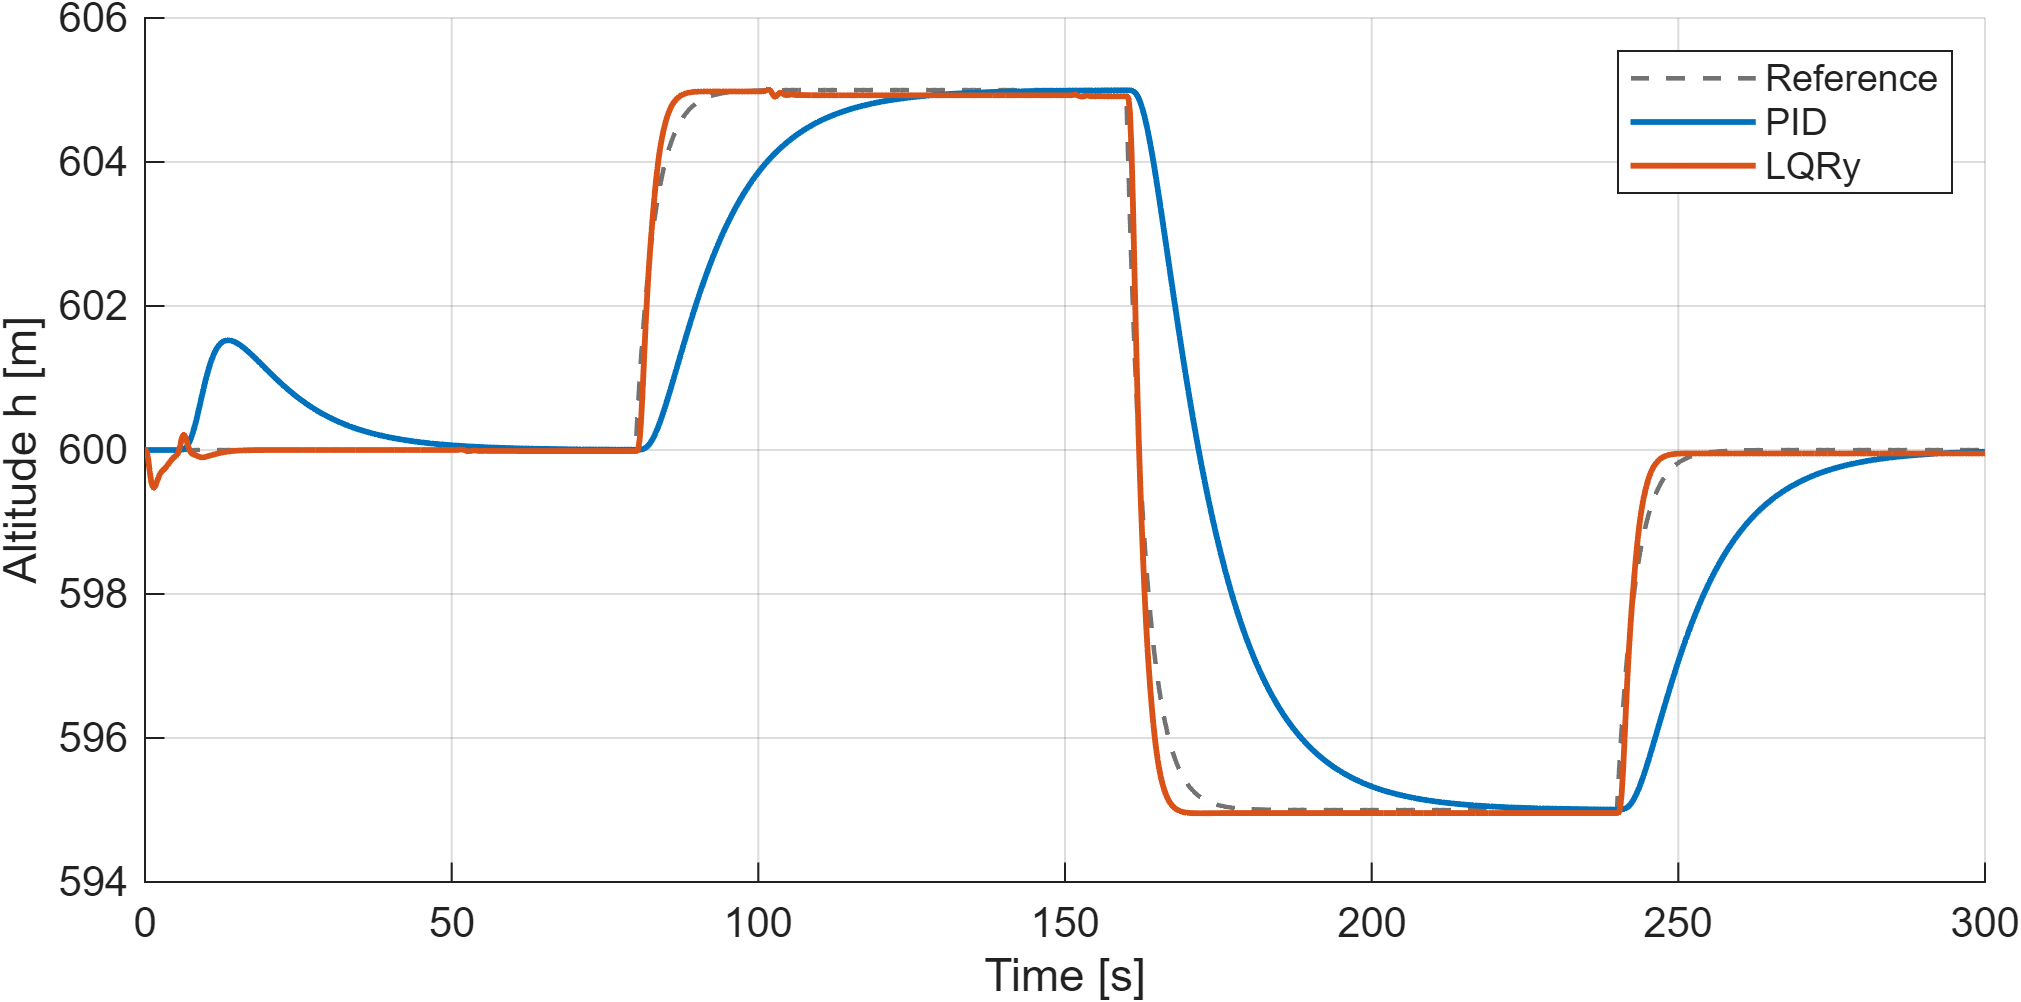
\includegraphics[width=\linewidth]{fig_alt_pid_lqry.png}
\caption{Altitude channel of the combined mission (SIL): reference,
PID, and LQRy on a single axis.}\label{fig:alt-single}\end{figure}
The roles observed in the earlier fixed-gain iteration of this
comparison are reversed: the gain-scheduled LQRy is now the fast,
high-bandwidth law --- it captures heading in ${\approx}13$\,s at the
cost of $16.4\%$ overshoot, and completes the airspeed and altitude
captures in ${\approx}6$\,s with essentially no overshoot --- while
the requirements-retuned PID is the smooth one, with zero overshoot on
every channel and settling times of 18--44\,s. Neither tuning
dominates: the LQRy buys speed at the cost of a heading-overshoot
requirement violation; the PID buys strict compliance at the cost of
bandwidth.

\begin{table}[!t]
\caption{Per-axis guidance captures (SIL, identical references),
metrics on the $+$step segment of each channel. OS = overshoot, $t_r$
= 10--90\% rise time, $t_s$ = 2\% settling time, $e_{ss}$ =
steady-state error.}
\label{tab:metrics}
\centering
\resizebox{\linewidth}{!}{%
\begin{tabular}{lcccccccc}
\toprule
 & \multicolumn{4}{c}{PID} & \multicolumn{4}{c}{LQRy} \\
Ch. & OS[\%] & $t_r$[s] & $t_s$[s] & $e_{ss}$[\%] & OS[\%] & $t_r$[s] & $t_s$[s] & $e_{ss}$[\%] \\
\midrule
$\VT$ & 0.0 & 9.48 & 18.0 & 0.00 & 0.0 & 3.04 & 5.8 & 0.00 \\
$\psi$ & 0.0 & 16.14 & 33.0 & 0.50 & 16.4 & 0.83 & 12.6 & 0.01 \\
$h$ & 0.0 & 23.37 & 44.4 & 0.06 & 0.6 & 3.44 & 5.9 & 0.19 \\
\bottomrule
\end{tabular}}
\end{table}

\begin{figure}[!t]
\centering
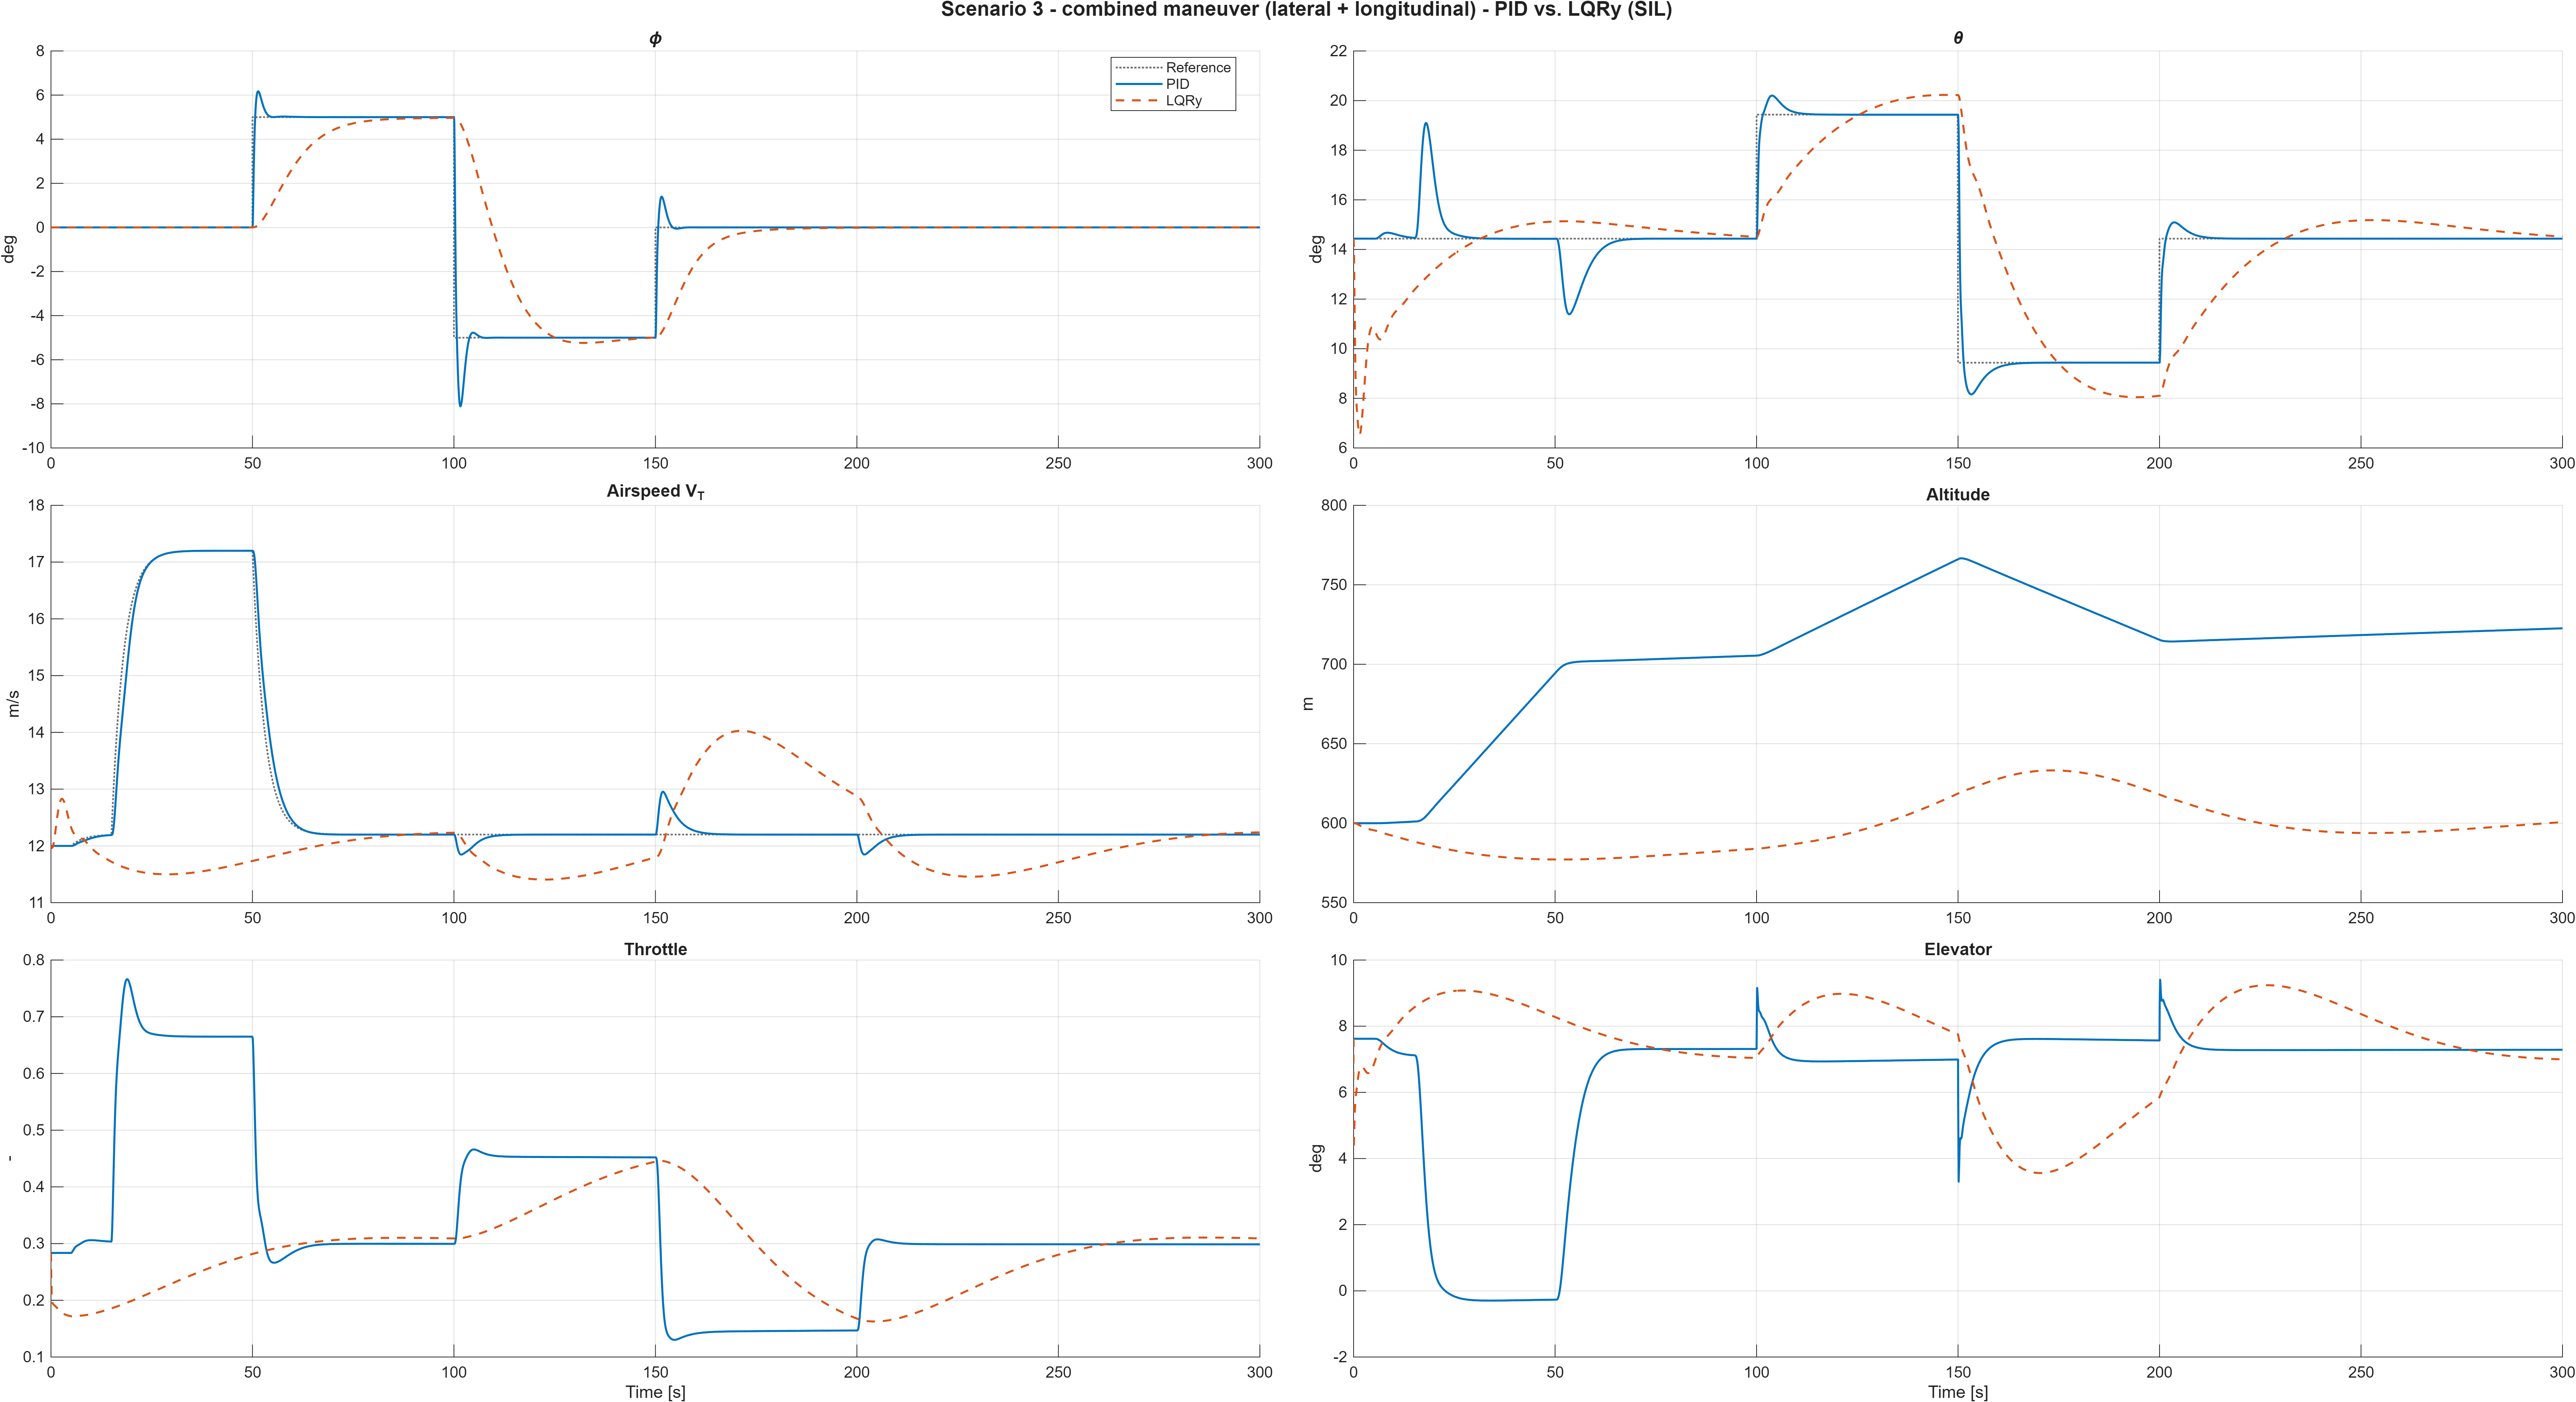
\includegraphics[width=\linewidth]{fig_cen_comb.png}
\caption{Scenario 4 (combined mission): PID vs.\ LQRy on the nonlinear
model, identical references.}
\label{fig:cen-comb}
\end{figure}

Table~\ref{tab:compliance} closes the loop with the requirements of
Section~\ref{sec:requirements}, evaluated on the guidance channels of
the combined mission. The PID meets every row. The LQRy settles far
inside the 60\,s limit on every channel (5.8--7.0\,s) and meets the
steady-state row, but violates the overshoot requirement on the
heading channel ($24.5\%$ against the $10\%$ line).

\begin{table}[!t]
\caption{Requirements compliance on the combined mission (SIL),
guidance channels, identical references.}
\label{tab:compliance}
\centering
\begin{tabular}{lcccccc}
\toprule
 & \multicolumn{3}{c}{PID} & \multicolumn{3}{c}{LQRy} \\
Requirement & $\VT$ & $\psi$ & $h$ & $\VT$ & $\psi$ & $h$ \\
\midrule
OS $<10\%$ & 0.0 & 0.0 & 0.0 & 0.2 & \textbf{24.5} & 0.2 \\
$t_s<60$\,s & 18.0 & 38.1 & 45.1 & 5.8 & 6.9 & 7.0 \\
$e_{ss}\le5\%$ & 0.00 & 0.72 & 0.07 & 0.00 & 0.00 & 1.75 \\
\bottomrule
\end{tabular}
\end{table}

The embedded (HIL) campaign of Section~\ref{sec:hil} was executed with
the \emph{earlier fixed-gain} LQRy build (Section~\ref{sec:lqry}), so
its LQRy-side numbers characterize that deployment rather than the
gain-scheduled law compared here; the PID-side SIL--HIL fidelity
results are unaffected.

% (Robustez movida para secao propria: sections/05_robustness.tex.
%  Remark de execution order movido, encurtado, para o fim de
%  sec:determinism no HIL — resolve o "???" da orientadora.)

\section{Robustness Study}
\label{sec:robustness}

The comparison of Section~\ref{sec:sil-comparison} holds for the nominal
plant --- the very model both controllers were designed on. This section
asks how much of that picture survives when the plant is no longer the
design model. The protocol is deliberately strict: \emph{only the plant
changes}. Both controllers keep the gains and trim commands of the nominal
design, and every run repeats the combined mission of
Section~\ref{sec:sil-comparison} ($\VT$ $12\!\to\!15.2$\,m/s at 5\,s,
heading doublet $\pm5^\circ$ at 50/100/150\,s, altitude doublet
$\pm5$\,m at 80/160/240\,s, 300\,s total) --- the same combined
mission, and the same per-axis reference set, used throughout
Section~\ref{sec:sil}. Four scenarios are considered,
spanning plausible-to-severe model uncertainty and an exogenous
disturbance: (A)~a severe model mismatch, replacing the complete
aerodynamic set by an independent identification of the same airframe;
(B)~the longitudinal half of that mismatch only, to isolate the origin of
the failure observed in~(A); (C)~a plausible identification uncertainty,
multiplying all 23 stability and control derivatives by 1.10; and (D)~wind
and gusts applied through the native disturbance inputs
of~\eqref{eq:inputvec}. Table~\ref{tab:robustness} summarizes the tracking
metrics; the degradation columns normalize each scenario by the same
controller's nominal performance, so that the two laws are compared
against themselves rather than against each other.

\begin{table*}[!t]
\caption{Robustness campaign: RMS tracking errors ($t>12$\,s) and
degradation relative to the nominal scenario (RMS scenario / RMS nominal).
Gains and trim always from the nominal design.}
\label{tab:robustness}
\centering
\begin{tabular}{llcccccc}
\toprule
 & & \multicolumn{3}{c}{RMS error} & \multicolumn{3}{c}{Degradation ($\times$ nominal)} \\
Scenario & Ctrl. & $\VT$ [m/s] & $\psi$ [$^\circ$] & $h$ [m] & $\VT$ & $\psi$ & $h$ \\
\midrule
Nominal & PID & 0.071 & 1.27 & 1.65 & --- & --- & --- \\
 & LQRy & 0.040 & 0.71 & 0.93 & --- & --- & --- \\
\addlinespace
(A) Severe mismatch & PID & 3.14 & 818.7 & 554.0 & 44.3 & 644 & 335 \\
 & LQRy & \multicolumn{6}{c}{diverges\textsuperscript{a}} \\
 & LQRy (fixed-gain)\textsuperscript{b} & 0.353 & 2.61 & 1.77 & 0.93 & 0.89 & 0.99 \\
\addlinespace
(B) Longitudinal only & PID & 0.081 & 1.28 & 113.8 & 1.14 & 1.01 & 68.9 \\
 & LQRy & 0.055 & 0.78 & 0.96 & 1.38 & 1.09 & 1.03 \\
\addlinespace
(C) All derivatives $\times1.10$ & PID & 0.073 & 1.28 & 1.65 & 1.03 & 1.01 & 1.00 \\
 & LQRy & 0.032 & 0.72 & 0.93 & 0.82 & 1.01 & 1.00 \\
\addlinespace
(D) Wind and gusts & PID & 0.104 & 2.24 & 2.55 & 1.46 & 1.76 & 1.54 \\
 & LQRy & 0.042 & 0.75 & 5.12 & 1.05 & 1.06 & 5.48 \\
\bottomrule
\multicolumn{8}{l}{\footnotesize\textsuperscript{a}The run terminates
at ${\approx}$55--60\,s, at the first heading-doublet reversal.}\\
\multicolumn{8}{l}{\footnotesize\textsuperscript{b}The earlier
fixed-gain bench build (Section~\ref{sec:hil}); degradation relative
to its own nominal run.}
\end{tabular}
\end{table*}

\subsection{Severe Model Mismatch}
\label{sec:rob-sato}
The perturbed plant replaces the nominal, flight-test-identified
aerodynamic set~\cite{angelo2026} by the complete alternative set
originally distributed with the nonlinear model
implementation~\cite{ferreira2019modeling,repo}, obtained through an
independent identification of the platform. The two sets differ
substantially --- the pitch-damping derivative $C_{m_q}$ by a factor of
4, the elevator effectiveness $C_{m_{\delta_e}}$ by 3.3, and the
lateral--directional set even changes the \emph{sign} of $C_{y_\beta}$
and $C_{y_p}$ --- so this scenario probes well beyond parametric
uncertainty: it is a structurally different aerodynamic description.

Under this mismatch \emph{both} laws lose the mission, each in its own
way. The PID enters a violent but bounded lateral oscillation: the
heading doublet triggers it, the heading error grows to
${\sim}2100^\circ$ (the aircraft flies repeated full circles), and the
altitude sinks by hundreds of meters (Table~\ref{tab:robustness}: RMS
heading error of $819^\circ$, altitude error of 554\,m). The
gain-scheduled LQRy fails harder: the run diverges outright before
60\,s, at the first heading-doublet reversal --- its high-bandwidth
lateral gains amplify the inverted-sign lateral--directional dynamics
instead of containing them: the heading error grows geometrically
across the reversal ($0.6^\circ$ at 51\,s, $17.7^\circ$ by 55\,s)
until the sideslip leaves the physical domain and the simulation
terminates. The contrast within the LQ family itself is the most
instructive result of the scenario: the earlier, softer
\emph{fixed-gain} LQRy iteration --- the build deployed on the bench
of Section~\ref{sec:hil} --- completes this same mission with
\emph{near-nominal} error (degradation of $0.89$--$0.99$,
Table~\ref{tab:robustness} and Fig.~\ref{fig:rob-sato}), so the same
structure spans the full range from unconditional survival to outright
divergence depending only on its tuning. Robustness to severe mismatch
is thus a property of the \emph{tuning}, not of the LQ structure per
se --- a point taken up in Section~\ref{sec:rob-discussion}.
\begin{figure}[!t]\centering
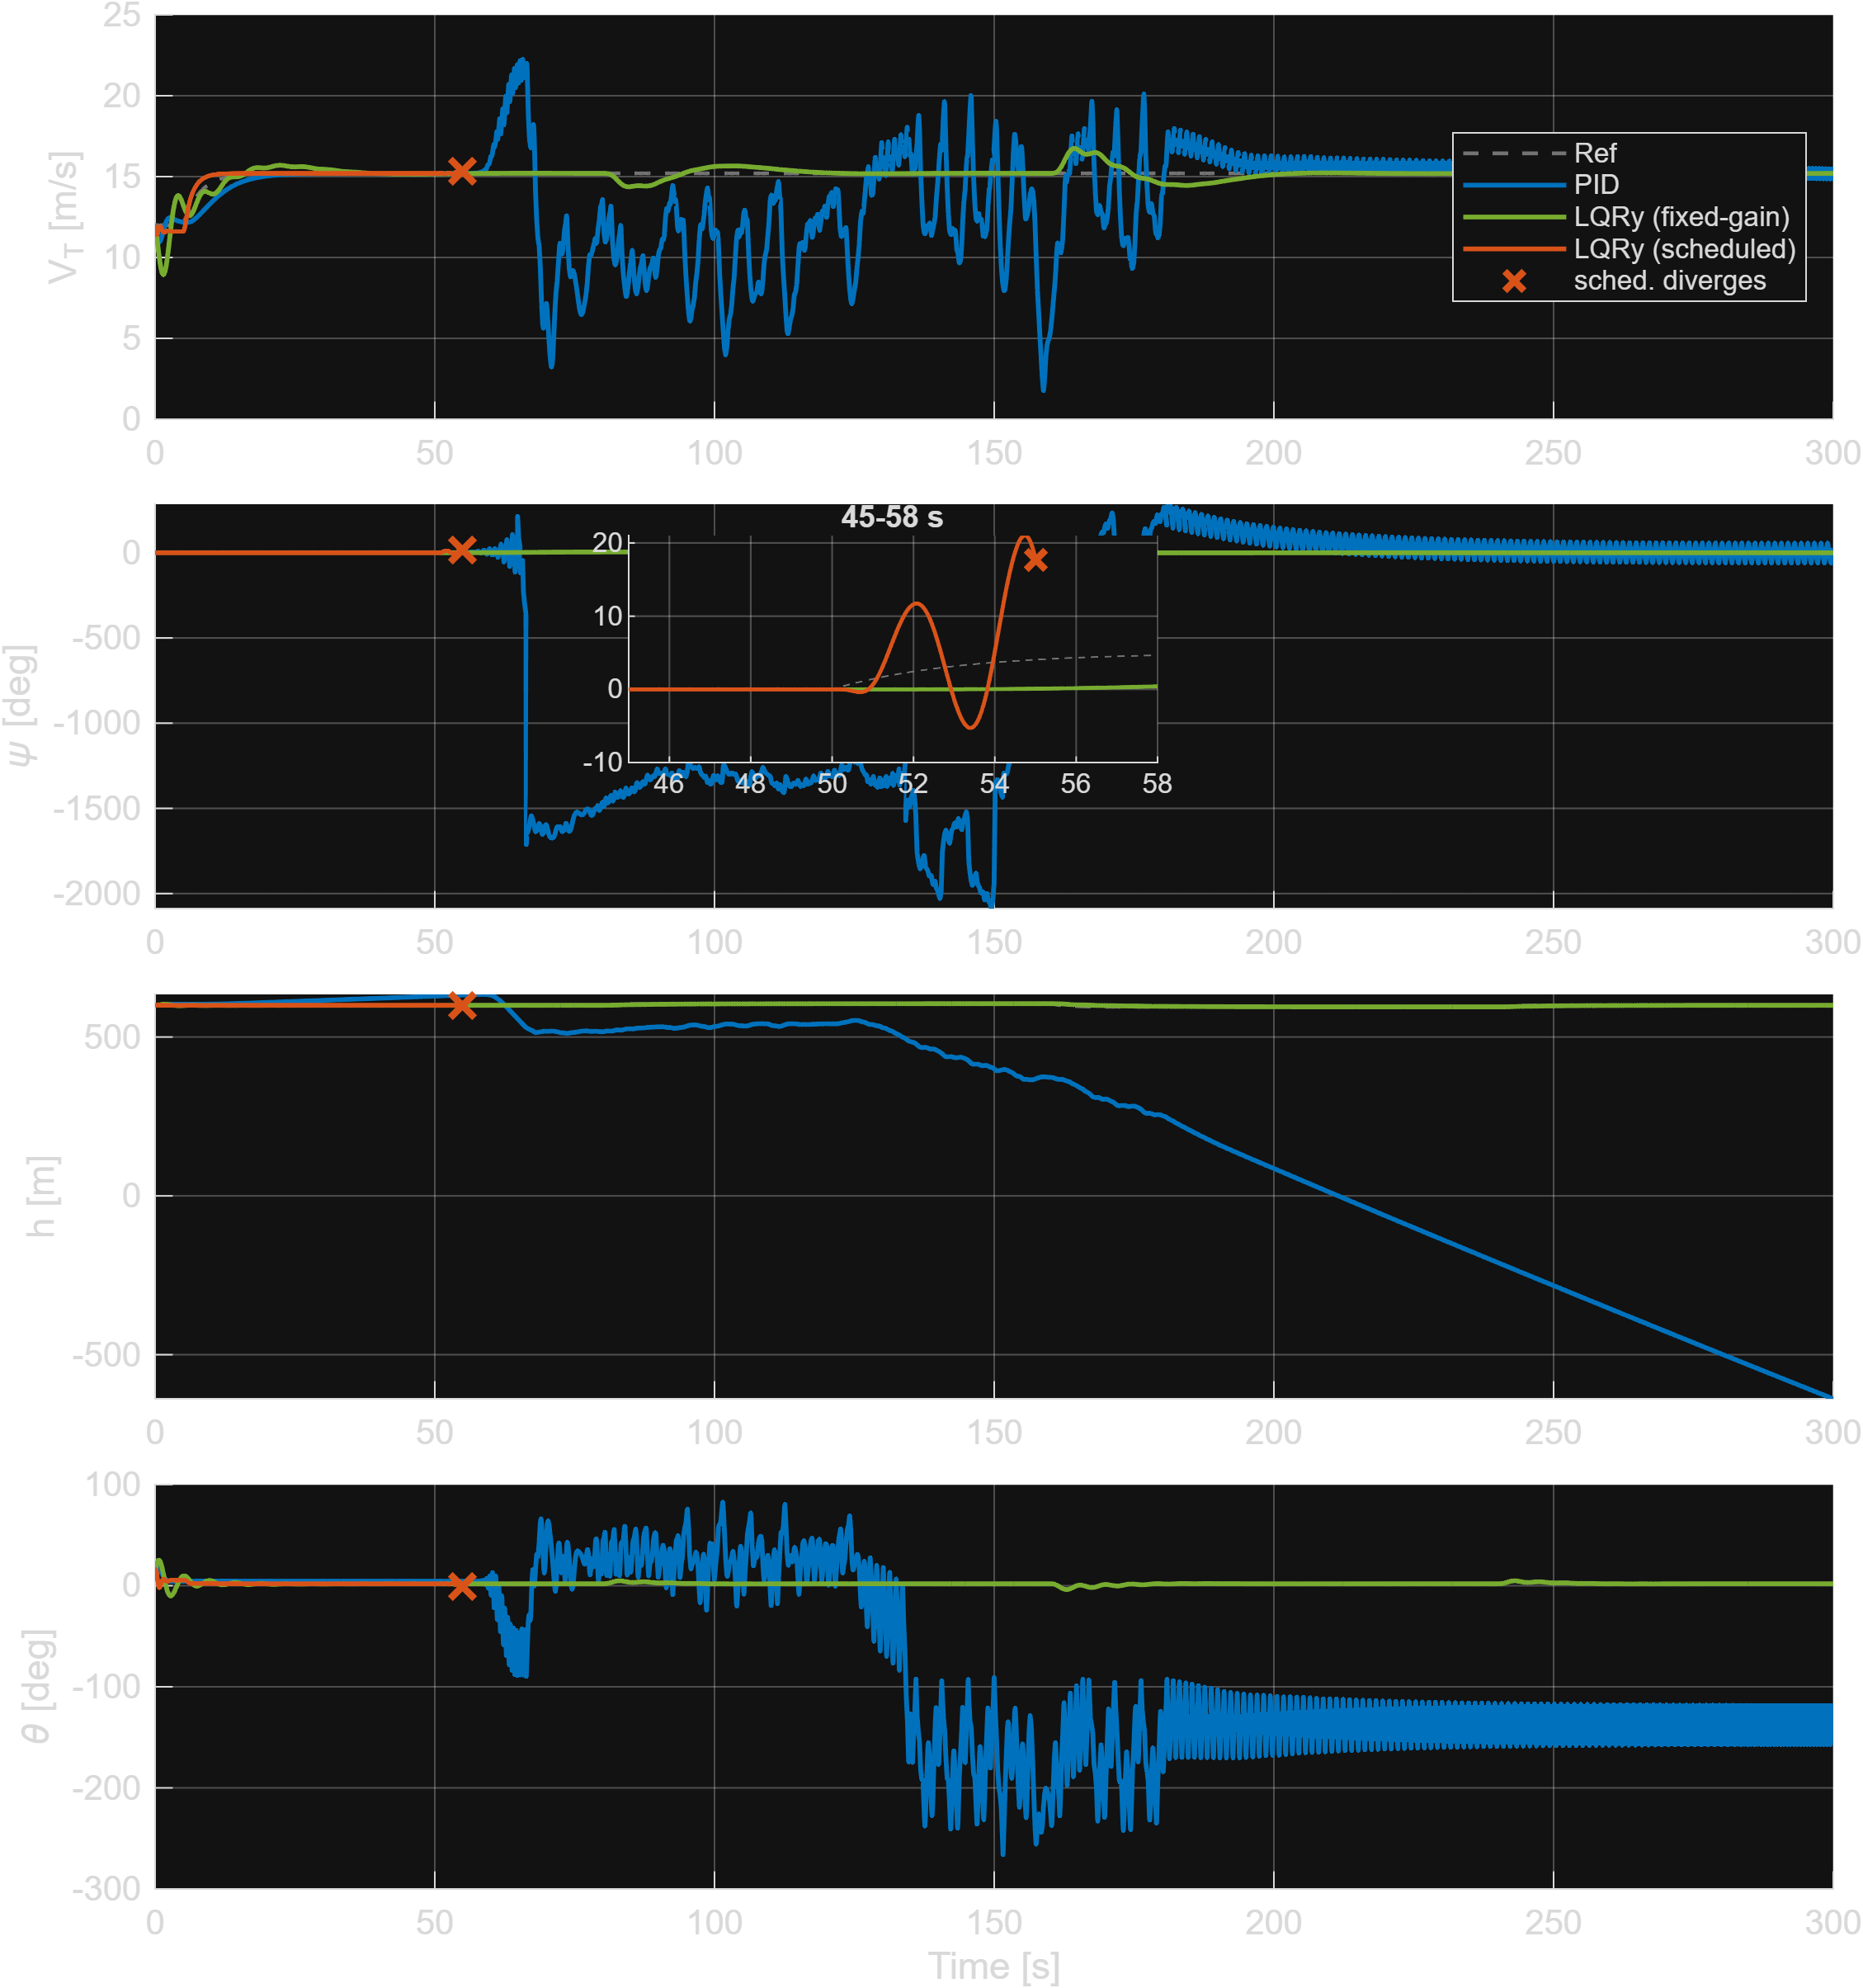
\includegraphics[width=\linewidth]{fig_rob_sato.png}
\caption{Scenario A (severe mismatch): combined mission on the
perturbed plant, nominal-design controllers. The fixed-gain LQRy
(bench build) completes the mission with near-nominal error; the
gain-scheduled LQRy diverges at the first heading reversal
($\times$ marker; inset: 45--58\,s).}\label{fig:rob-sato}\end{figure}

\subsection{Isolating the Origin: Longitudinal Mismatch Only}
\label{sec:rob-satoL}
Scenario B replaces only the \emph{longitudinal} derivatives by the
mismatched set, keeping the nominal lateral--directional model. Both
laws now complete the mission, which identifies the
lateral--directional half of the mismatch --- with its sign inversions
--- as what defeats them both in Scenario~A. The LQRy stays near
nominal in every channel (degradation of 1.03--1.38). The PID
maintains heading and airspeed at nominal levels (degradation of 1.01
and 1.14), but the longitudinal mismatch alone is not benign for it:
the altitude channel degrades by a factor of 69 (RMS 113.8\,m),
a steady drift of the altitude hold. The mechanism is specific: the
$\theta^{ref}$ clamp of $\pm10^\circ$ (Section~\ref{sec:pid}), sized for
the control authority of the nominal model, leaves the altitude loop
without enough authority on the perturbed plant, and the loop drifts
without ever diverging.
\begin{figure}[!t]\centering
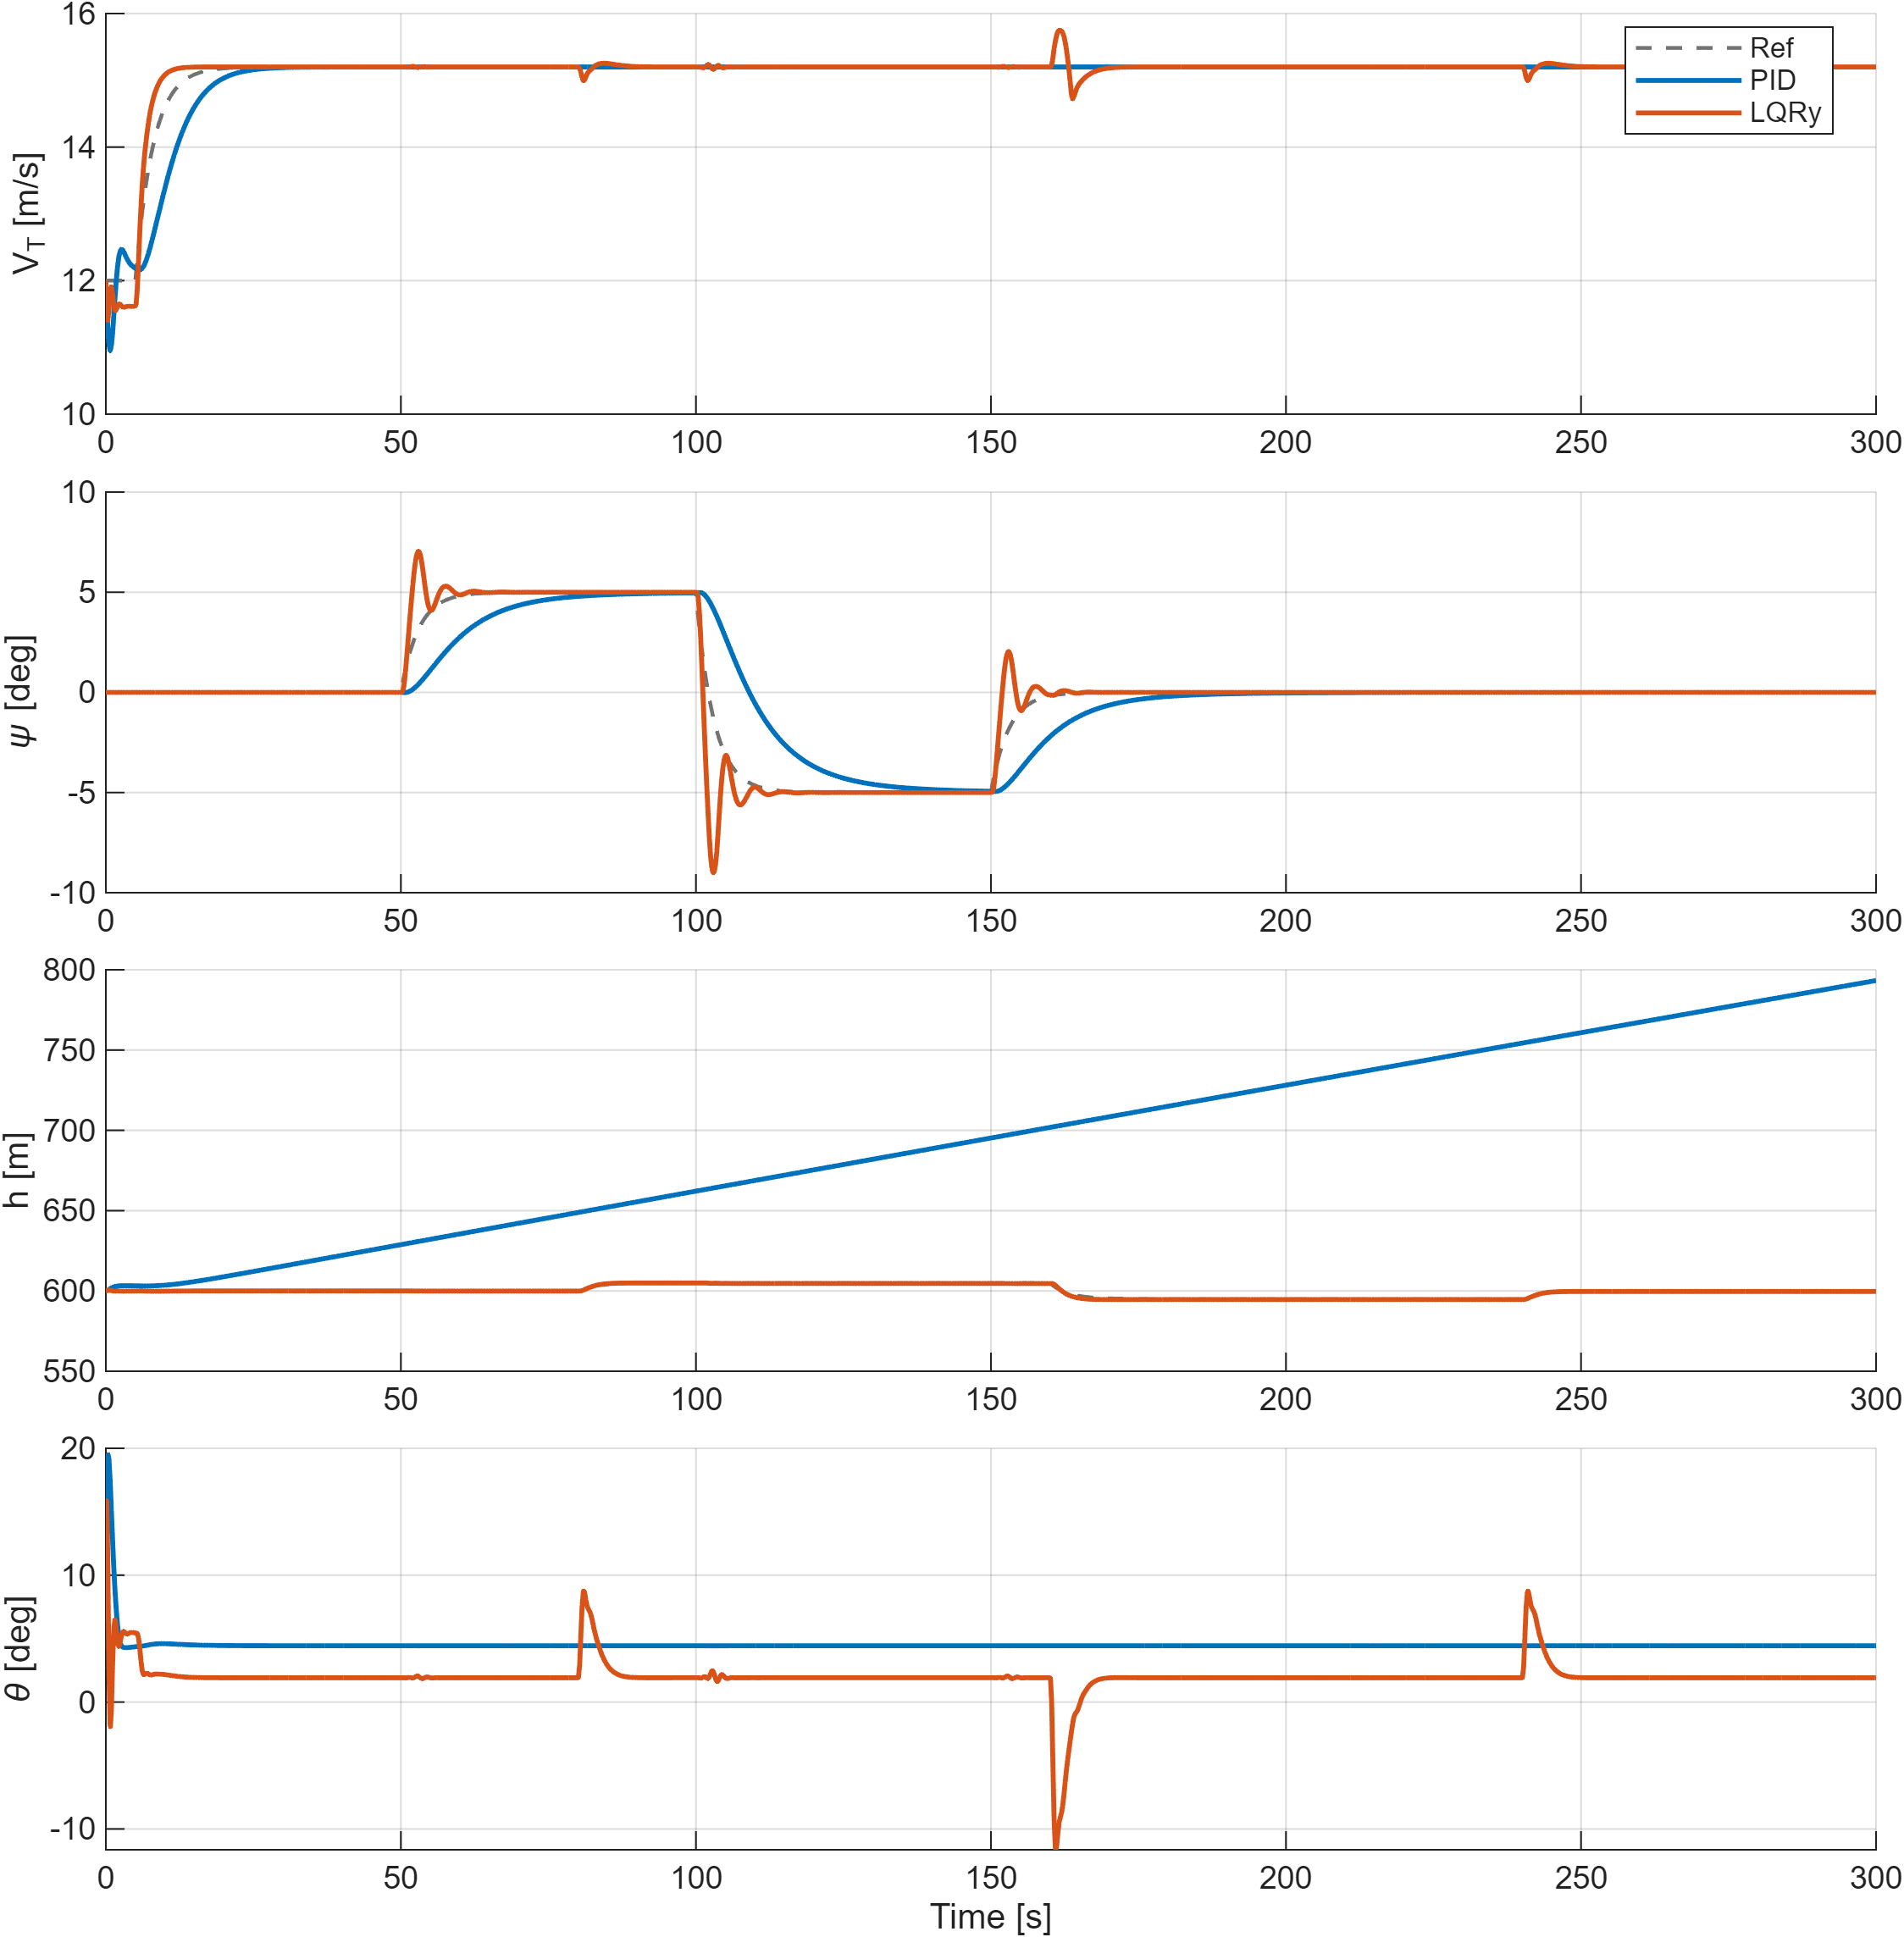
\includegraphics[width=\linewidth]{fig_rob_satoL.png}
\caption{Scenario B (longitudinal mismatch only).}
\label{fig:rob-satoL}\end{figure}

\subsection{Plausible Identification Uncertainty}
\label{sec:rob-pert}
Scenario C multiplies all 23 stability and control derivatives by 1.10
--- a uniform $+10\%$ multiplicative perturbation with preserved signs,
representative of a realistic identification error, in the spirit of
the perturbed-derivative robustness campaigns of the fixed-wing UAV
literature~\cite{safwat2019design}. Both controllers are
insensitive to it: every degradation factor lies between 0.82 and 1.03,
and the responses are visually indistinguishable from the nominal runs.
Within plausible identification uncertainty, \emph{both} designs are
robust; the contrast between them only appears under the severe,
sign-changing mismatch of Scenarios A--B.

\subsection{Wind and Gusts}
\label{sec:rob-vento}
Small, low-speed fixed-wing UAVs are disproportionately sensitive to
atmospheric disturbance --- gust velocities are a large fraction of
their airspeed~\cite{mohamed2014fixedwing} --- so no comparison of
flight controllers for this class is complete without a wind scenario.
Scenario D perturbs the nominal plant through the wind inputs
of~\eqref{eq:inputvec}: a 4\,m/s tailwind ramped in over 20--25\,s, two
lateral $1-\cos$ gusts of $\pm3$\,m/s (55--65\,s and 105--115\,s, timed
over the heading doublet), and two vertical $1-\cos$ gusts of
$\pm2$\,m/s (85--95\,s and 165--175\,s, timed over the altitude
doublet). The $1-\cos$ profile is the classical discrete-gust
idealization~\cite{hoblit1988gust}, retained to this day in the gust
conditions of certification regulations~\cite{far25341}; deterministic
discrete gusts (rather than stochastic Dryden or von K\'arm\'an
turbulence~\cite{milf8785c1980,milhdbk1797}) keep the scenario exactly
reproducible run to run, consistent with the deterministic-bench
philosophy of Section~\ref{sec:hil}. Both controllers remain stable
and complete the mission with moderate peak errors. The LQRy shows the
largest single degradation of the scenario --- altitude RMS
$\times5.48$ (5.12\,m) --- while the PID degrades most in heading
under the lateral gusts (RMS $\times1.76$, peak error $12.9^\circ$).
In \emph{absolute} terms, however, the LQRy still tracks heading more
tightly under the gusts (RMS $0.75^\circ$ versus $2.24^\circ$) but
pays in altitude (RMS 5.12\,m versus 2.55\,m). Neither controller
approaches loss of control.
\begin{figure}[!t]\centering
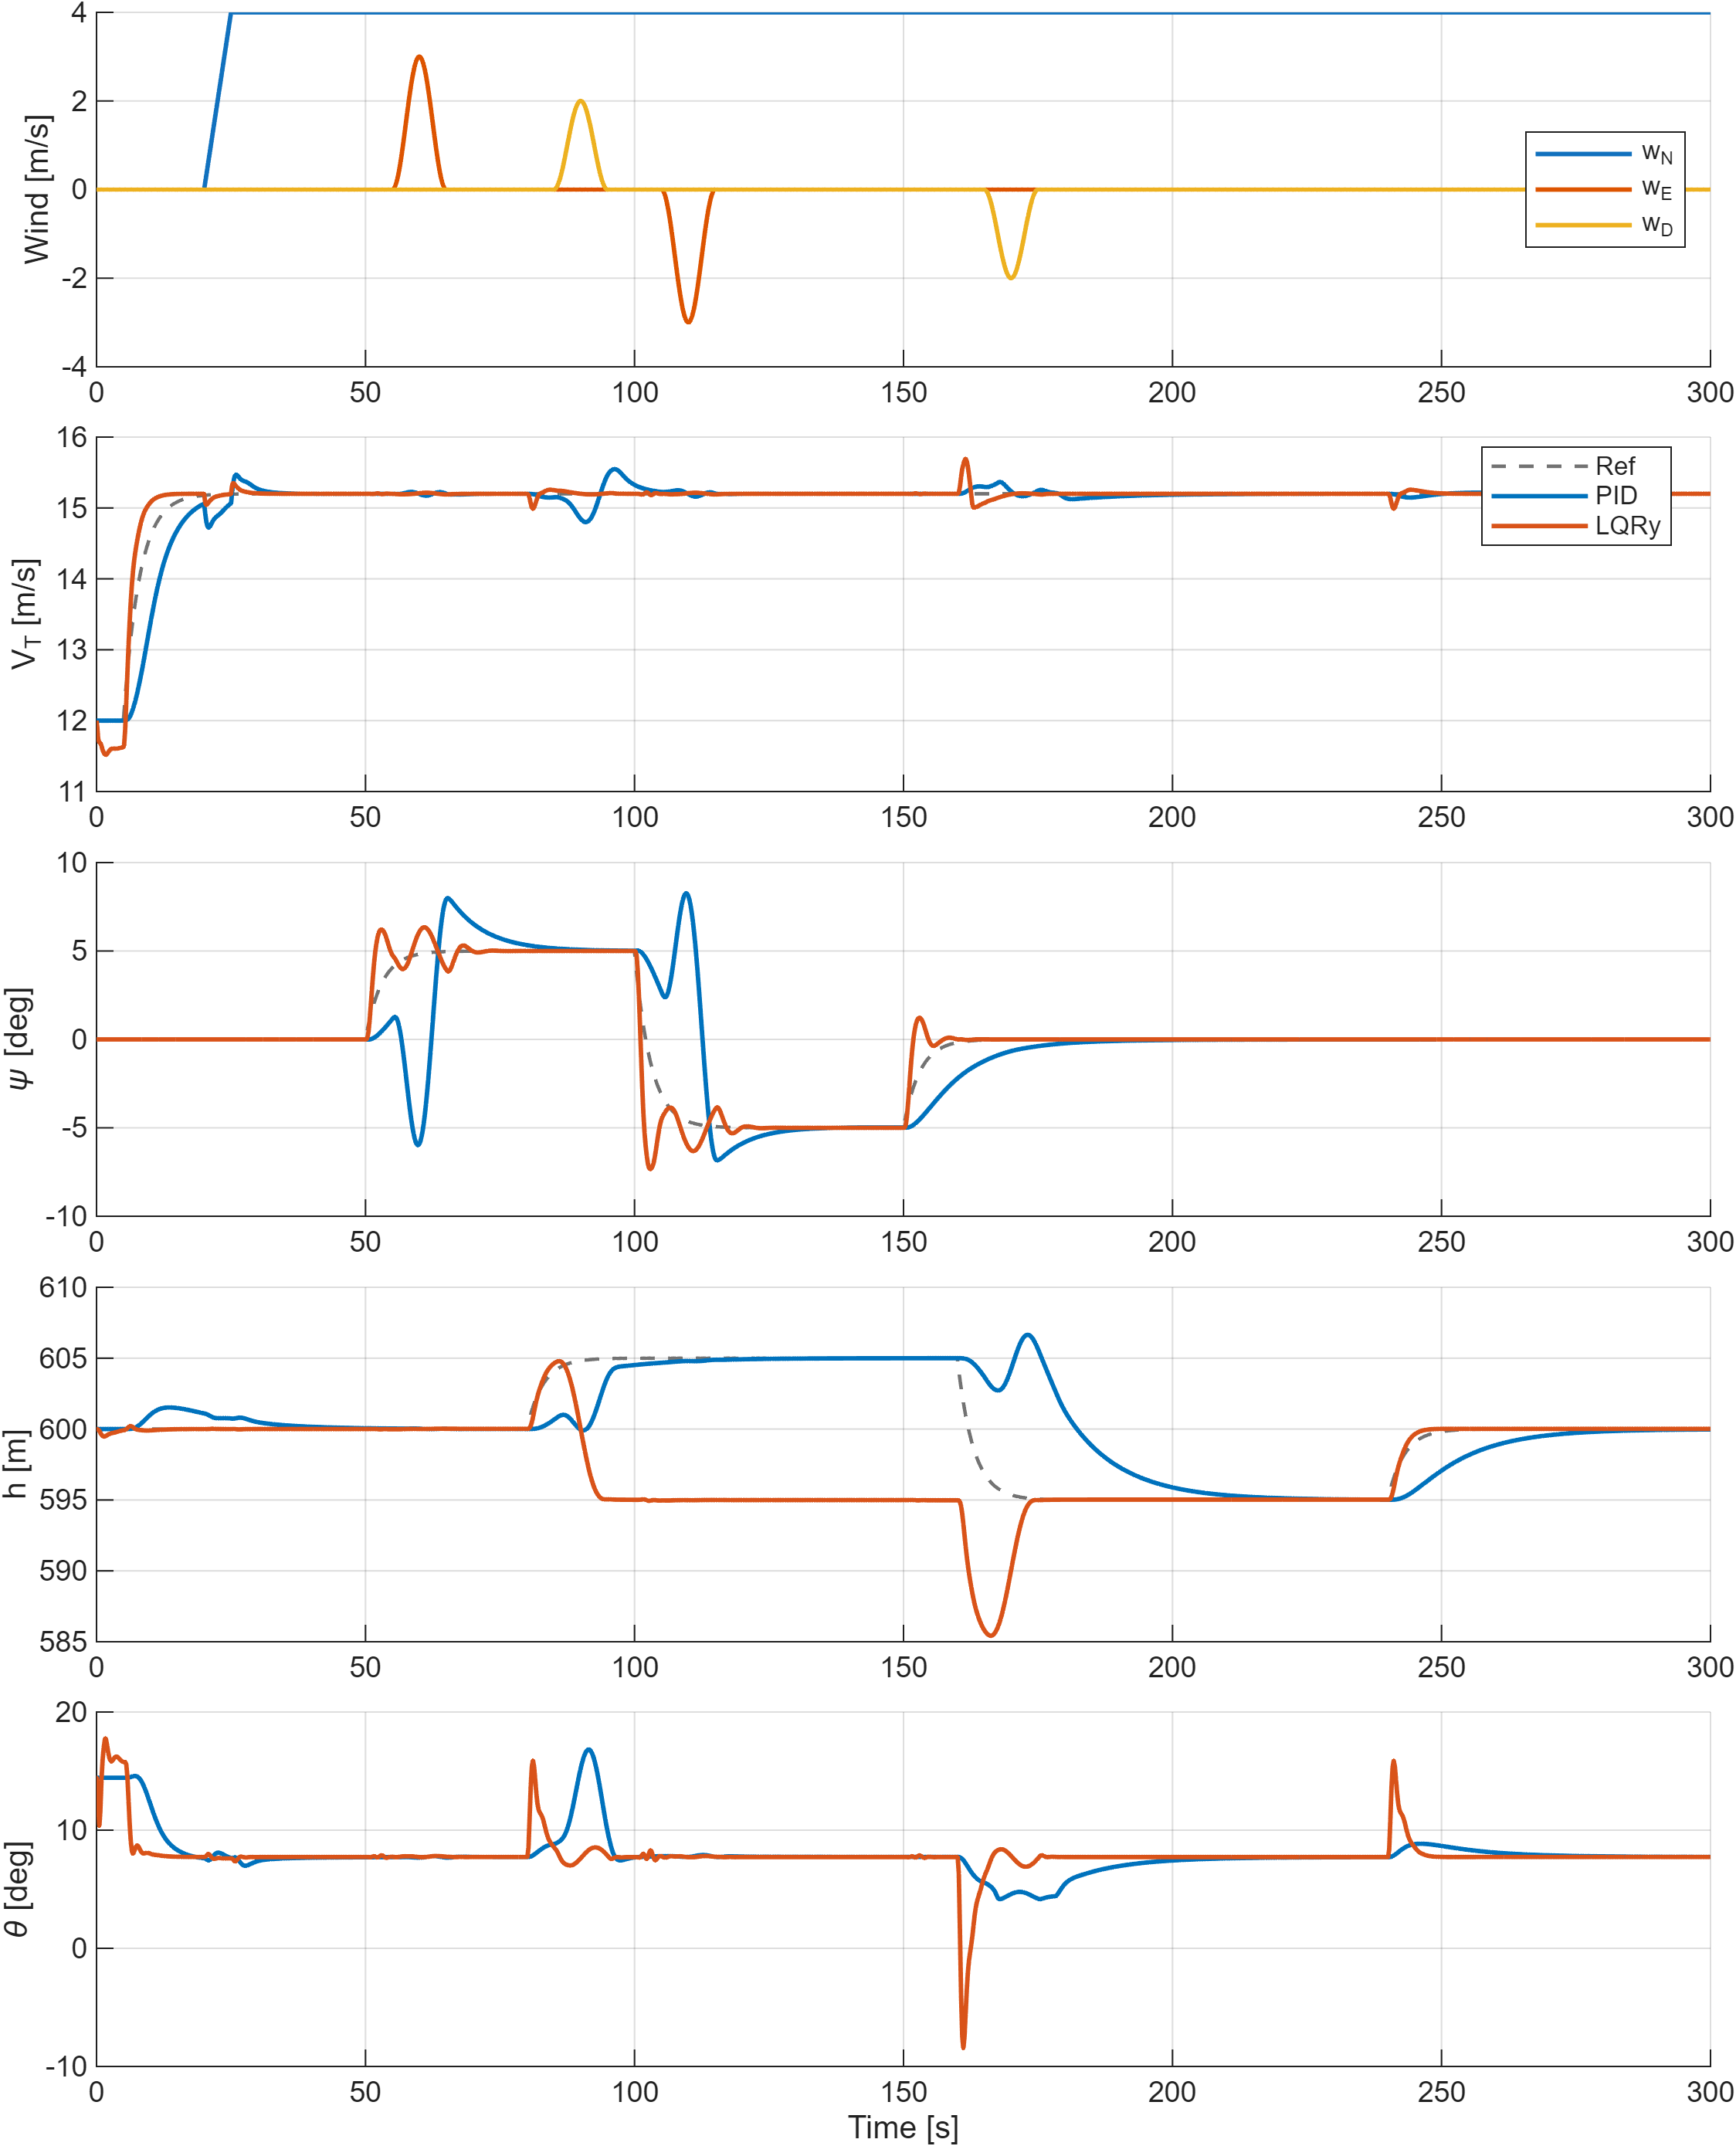
\includegraphics[width=\linewidth]{fig_rob_vento.png}
\caption{Scenario D (wind and gusts): wind profile and closed-loop
responses.}\label{fig:rob-vento}\end{figure}

\subsection{Discussion}
\label{sec:rob-discussion}
The study still exposes \emph{complementary} weaknesses, but
redistributed with respect to the earlier fixed-gain iteration of this
comparison. The severity of the model mismatch now defeats \emph{both}
laws: the cascade PID because a sign change in the lateral derivatives
invalidates its fixed loop shapes, and the gain-scheduled LQRy because
its high-bandwidth lateral gains turn the same sign change into
outright divergence. That an earlier, softer fixed-gain LQRy iteration
tolerated the same scenario is consistent with the gain and phase
margins classically guaranteed for LQ state
feedback~\cite{safonov1977gain} being lost under output feedback in
general~\cite{doyle1978guaranteed}: whatever mismatch tolerance an LQ
output-feedback design exhibits is an empirical property of the
specific tuning rather than a theorem, and aggressive tuning spends
it. The discriminators between the two laws lie elsewhere: under the
longitudinal-only mismatch (B) the PID silently starves an outer loop
through a clamp sized for the nominal plant while the LQRy stays near
nominal, and under wind (D) the LQRy concedes altitude where the PID
holds firm; within plausible uncertainty (C) both are robust.
Robust-control syntheses that shape this trade-off explicitly have
been pursued for small fixed-wing UAVs in our own research
context~\cite{abdulhamid2016robusto}; here the point is narrower:
between the two \emph{standard} laws compared, neither dominates under
uncertainty, and which weakness matters more depends on whether the
dominant threat is model error or atmospheric disturbance.

\section{Hardware-in-the-Loop Development}
\label{sec:hil}
HIL simulation is the established bridge between simulation and
flight for UAV autopilots~\cite{jung2007hil,cai2009design}, and the
bench lineage of our group runs from the Pegasus real-time HIL
architecture~\cite{bittar2012pegasus} through X-Plane-based attitude
HIL~\cite{bittar2014hil} to the fixed-wing autopilot bench of
Santos~\cite{santos2018}. This section describes the present
incarnation: a lockstep serial bench in which the embedded controller
is the auto-generated production code.

\subsection{Controller Discretization}
\label{sec:discretization}
Both controllers are discretized at $T_s = 10$\,ms directly in Simulink
(automatic conversion of the compensators to their discrete-time forms;
the washout filter via Tustin transformation), producing single-rate
discrete models suitable for code generation. The discretized PID was
verified against the continuous design on the nonlinear model, with an RMS
deviation below $0.1\%$ of each command amplitude --- discretization is
\emph{not} a significant error source at this sample rate, as quantified
in Section~\ref{sec:sensitivity}.

\emph{A practical note on output saturation:} applying the automatic
conversion to the complete control loop with the output saturation blocks
included did not yield a working discrete model. The procedure adopted was
to discretize the control law alone and to re-insert the saturations
\emph{after} discretization. In the deployment reported here the
saturation limits (throttle in $[0,1]$, surfaces at $\pm 25^\circ$) are
enforced in the embedded C code, mirroring the host-side limits exactly.

\subsection{HIL Architecture}
\label{sec:hil-arch}
Fig.~\ref{fig:hil-loop} shows the architecture. The discrete controller is
translated to C by Simulink Embedded Coder (\texttt{ert.tlc}, ARM
Cortex-M, double precision) --- the automatic-code-generation workflow
of model-based aerospace software
practice~\cite{erkkinen2006automatic,erkkinen2009model} --- and
embedded in an STM32 microcontroller running FreeRTOS --- a class of
target for which HIL validation remains an active
topic~\cite{laabousse2025advanced}. The host PC runs \emph{only} the nonlinear plant, the
reference generation, and the serial interface. Host and target exchange
one frame per controller period over a 460\,800-baud serial link:
16 single-precision floats to the target (states, filtered references, and
mode switches) and 4 floats back (throttle, elevator, aileron, rudder),
delimited by a fixed header (\texttt{0xDE 0xAD}) and terminator.

The link operates in \emph{lockstep}, the mechanism by which
simulator and autopilot advance strictly by exchanged messages to make
runs deterministic and reproducible --- standard practice in
simulation stacks such as PX4~\cite{px4lockstep}: the plant blocks at
each 10\,ms simulation step until the controller reply arrives, so
simulated time advances only upon a completed exchange. Every HIL sample therefore
corresponds one-to-one to a SIL sample --- the comparison is free of
timing jitter by construction.

Two aspects of the campaign design are worth stating explicitly, as they
are what make the SIL and HIL results directly comparable:
\begin{itemize}
  \item \emph{Single source of references.} One script generates both the
        SIL and the HIL runs of every flight case, so the two campaigns
        cannot drift apart in their reference definitions.
  \item \emph{Mode selection over the link.} The three flight-mode
        switches travel in the frame rather than being compiled into the
        firmware, so a single binary serves all flight cases of the PID
        deployment and the target is never reprogrammed mid-campaign
        (the LQRy deployment deviates from this, as noted in
        Section~\ref{sec:campaigns}).
\end{itemize}

\begin{figure}[!t]
\centering
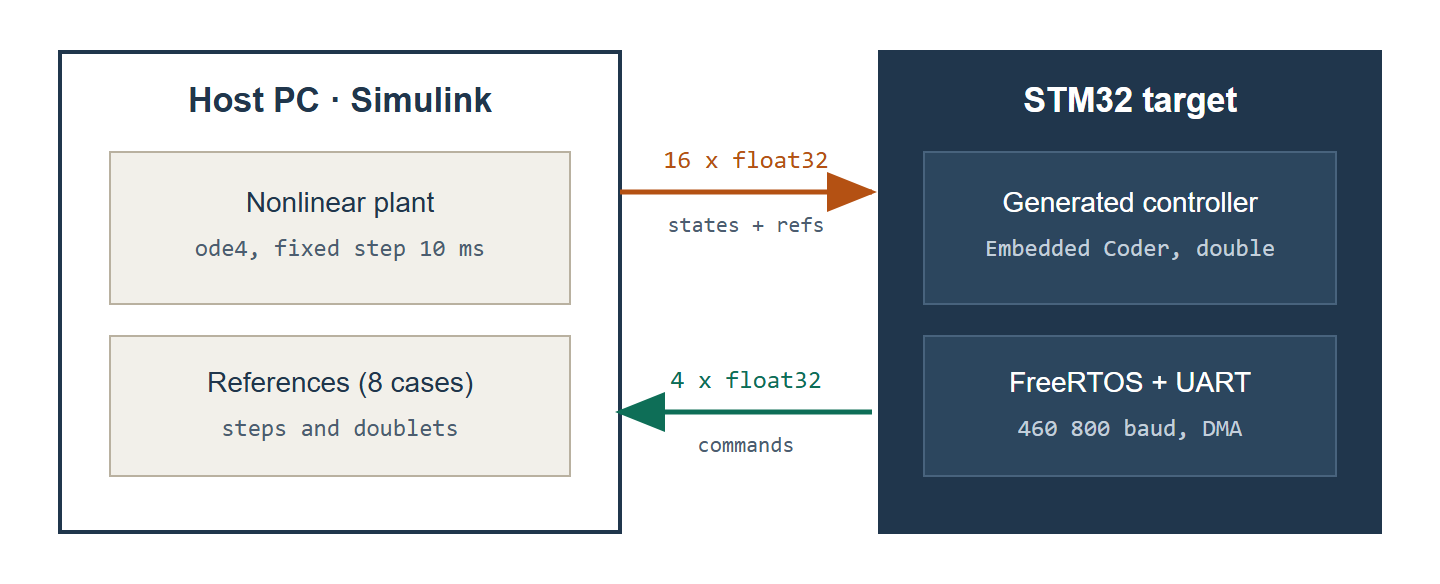
\includegraphics[width=\linewidth]{hil_loop.png}
\caption{HIL loop in lockstep: nonlinear plant on the host, generated
controller code on the STM32, binary serial frames at each 10\,ms step.}
\label{fig:hil-loop}
\end{figure}

\subsection{Link and Chain Validation}
Before any campaign, each element of the chain was validated
independently: (i) serial echo at 460\,800 baud with zero errors;
(ii) a frame-level test in which the embedded controller response to 200
known input frames matched the simulated discrete controller to within
$4\times10^{-8}$ (the single-precision quantization of the bus); and
(iii) the discretization check of Section~\ref{sec:discretization}.

\subsection{Determinism of the Lockstep Loop}
\label{sec:determinism}
A lockstep HIL loop built from double-precision arithmetic on both sides,
with single-precision quantization only on the wire, has no source of
run-to-run variability: there is no timing race, no dropped-sample
interpolation, and no floating-point reduction whose order can change.
The loop should therefore be \emph{bit-deterministic}.

We verified this property directly. The generated LQRy controller was
compiled and executed on a microcontroller model \emph{different} from the
one used in an earlier execution of the same code (STM32F303 versus
STM32F411, different core configurations and clock trees), driving the same
host model. Over a full 300-second flight case, the two executions
produced \emph{bit-identical} outputs on all recorded channels (maximum
difference identically zero, Fig.~\ref{fig:replica}); repeating additional
flight cases of the campaign reproduced the same result.

\begin{figure}[!t]
\centering
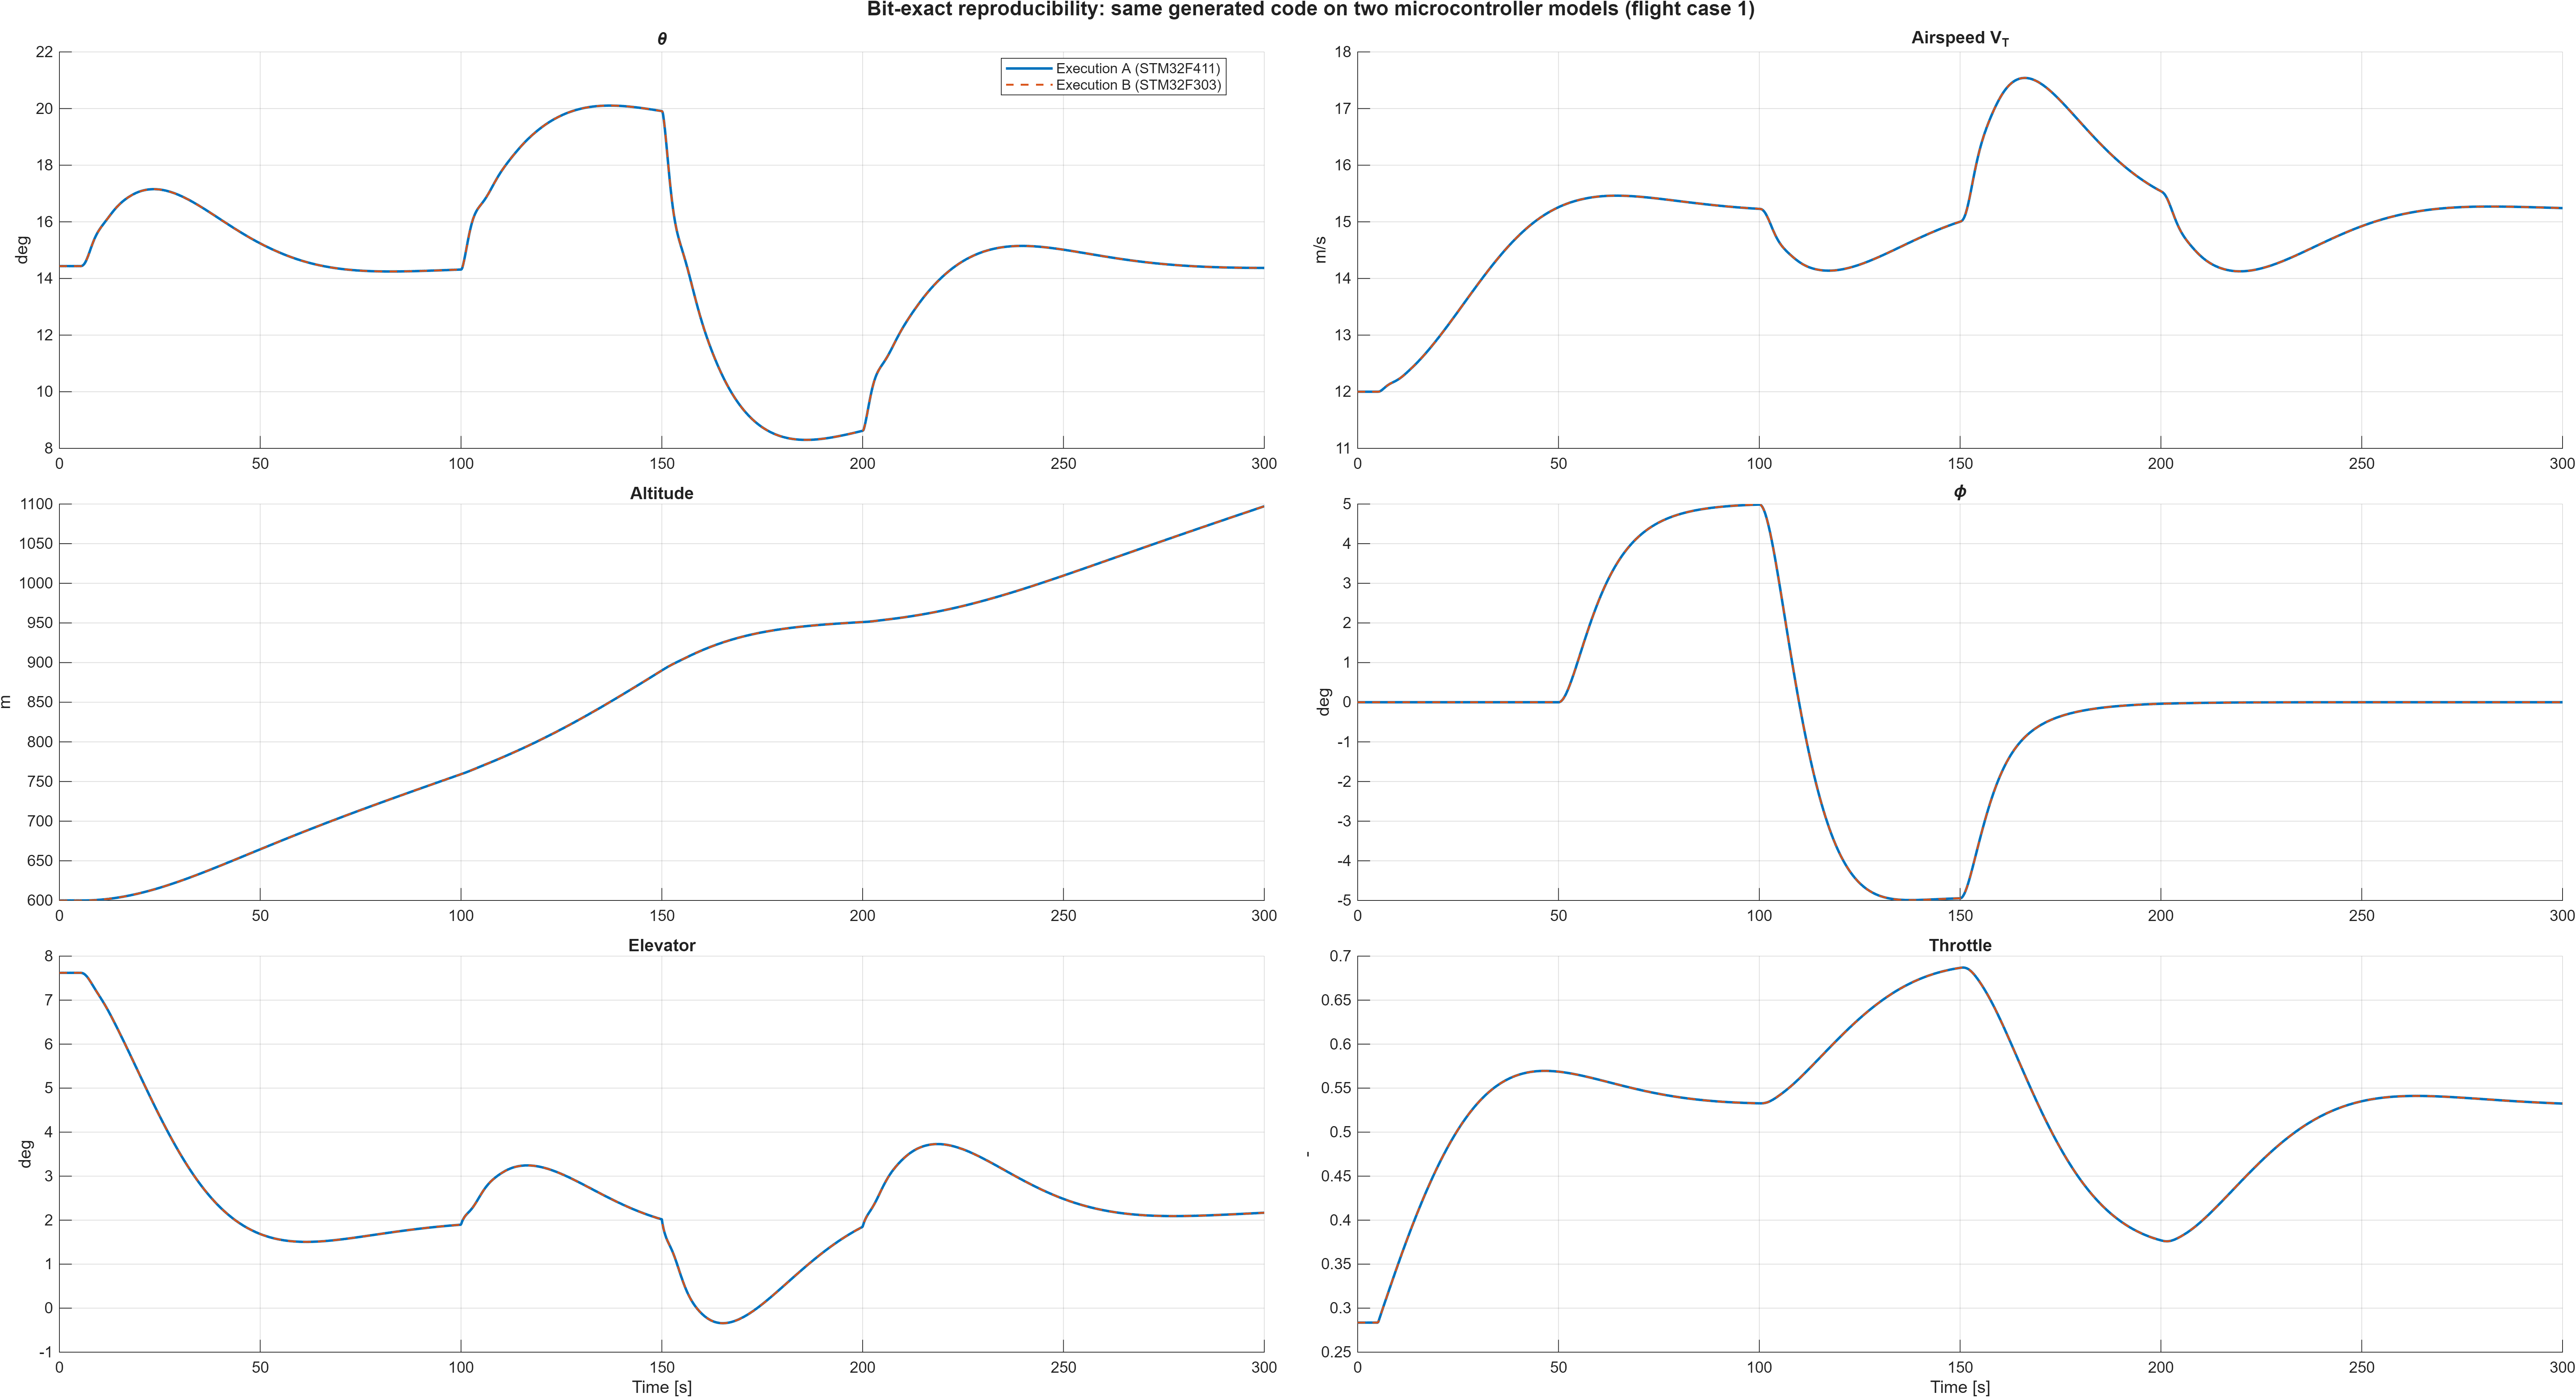
\includegraphics[width=\linewidth]{replica_caso1.png}
\caption{Bit-exact reproducibility: the same generated controller code
executed on two different microcontroller models over a 300-second flight
case. Maximum difference across all channels is identically zero.}
\label{fig:replica}
\end{figure}

This is a useful property for a validation bench, and not merely a
curiosity. Because the loop contributes no noise of its own, \emph{any}
deviation observed between two runs is attributable to a deliberate change
in the setup, which makes the bench a measuring instrument rather than a
source of scatter. It also means that a campaign can be reproduced exactly
by a third party, on different hardware, from the archived code and
reference definitions --- a stronger form of reproducibility than the
usual statistical agreement. The sensitivity study of the next subsection
relies on this: each experiment changes exactly one factor, and the
resulting difference is entirely due to that factor.

This determinism also settles a practical concern of embedded
deployment: block \emph{execution order} in a graphical model can, in
principle, alter the generated real-time code with respect to the
simulation. Here, with both controllers auto-generated from single-rate
discrete models, the cross-MCU bit-exactness rules out target-side
nondeterminism, and the quantization-floor SIL--HIL residual of the
synchronized PID deployment (Section~\ref{sec:campaigns}) bounds any
execution-order effect at the level of the bus quantization itself.

\subsection{Sensitivity of SIL--HIL Agreement}
\label{sec:sensitivity}
Deploying a control law on an embedded target involves a number of
implementation choices whose effect on SIL--HIL agreement is rarely
quantified. Exploiting the determinism established above, we injected each
factor individually into the validated PID bench and measured the
resulting discrepancy against the clean SIL run
(Table~\ref{tab:sensitivity}). All experiments use flight case 1; the
baseline row is the unmodified bench.

\begin{table}[!t]
\caption{Sensitivity of SIL--HIL agreement: each factor injected
individually into the validated bench (RMS vs.\ the clean SIL run, flight
case 1).}
\label{tab:sensitivity}
\centering
\begin{tabular}{lcc}
\toprule
Factor & $\theta$ [$^\circ$] & $h$ [m] \\
\midrule
Baseline (unmodified bench) & 0.030 & 0.09 \\
S1: start-up desynchronization (7\,s) & 0.014 & 0.07 \\
S2: airspeed reference mismatch (3\,m/s) & 0.447 & 258 \\
S3: controller discretization & 0.003 & 0.001 \\
S4: 1\% frame loss & 0.032 & 1.30 \\
\bottomrule
\end{tabular}
\end{table}

The ranking is informative, and in part counter-intuitive:

\subsubsection{Reference consistency dominates (S2)} An airspeed reference
differing by 3\,m/s between the SIL and HIL campaigns --- a plausible
outcome whenever the two campaigns are configured from separate scripts
--- produces a 258\,m RMS altitude discrepancy. This is not a fidelity
loss of the HIL chain at all: it is a comparison between two different
flight conditions. It is, by two orders of magnitude, the largest effect
measured, which motivates the single-source-of-references design of
Section~\ref{sec:hil-arch}.

\subsubsection{Start-up desynchronization leaves a persistent residual (S1)}
Embedded controllers commonly hold their integrators in reset until the
communication link engages, so the target starts from the trim command
while the simulated controller starts from its initial states and produces
an initial transient. The two trajectories then differ over the first
seconds and, in modes where an outer loop is open, that difference is
integrated and never recovered. Synchronizing the two start-ups --- as
done in the PID deployment --- removes this term; leaving them
unsynchronized leaves a residual that no amount of link quality can
remove.

\subsubsection{Frame loss is benign at low rates (S4)} Discarding 1\% of
the controller replies at random --- each discarded reply is replaced by
holding the previous command for that step, so the lockstep timing is
preserved --- degrades altitude agreement to 1.30\,m
but leaves attitude essentially unaffected, since the actuator rate limits
and the airframe dynamics filter isolated command glitches. This is
reassuring for links less reliable than the one used here.

\subsubsection{Discretization is negligible (S3)} The usual first suspect
--- the continuous-to-discrete conversion of the control law --- accounts
for $0.003^\circ$ in attitude and $10^{-3}$\,m in altitude at
$T_s=10$\,ms, three orders of magnitude below the reference-consistency
term.

\subsection{Embedded Campaign Results}
\label{sec:campaigns}
Eight flight cases (all combinations of the three mode switches, with
doublets on attitude/heading and steps on airspeed/altitude, 300\,s each)
were executed in SIL and HIL for both controllers, from a single script
per controller.

\subsubsection{PID} Table~\ref{tab:pid-silhil} reports the RMS SIL--HIL
discrepancy ($t>12$\,s). The residual reaches the quantization floor:
pitch attitude within $0.011^\circ$ in the worst case, altitude within
2.75\,m only where the altitude loop is open (integrated drift), and
essentially zero elsewhere. Fig.~\ref{fig:pid-c1} illustrates case~1: the
SIL and HIL traces are indistinguishable at plot scale.

\begin{table}[!t]
\caption{PID: RMS SIL--HIL discrepancy per flight case ($t>12$\,s).}
\label{tab:pid-silhil}
\centering
\begin{tabular}{lcccc}
\toprule
Case & $\theta$ [$^\circ$] & $\VT$ [m/s] & $h$ [m] & $\phi$ [$^\circ$] \\
\midrule
1 & 0.0028 & 0.0009 & 0.089 & $\sim$$10^{-6}$ \\
2 & 0.0007 & 0.0002 & 0.004 & $\sim$$10^{-6}$ \\
3 & 0.0035 & 0.0011 & 2.75  & $\sim$$10^{-6}$ \\
4 & 0.0007 & 0.0002 & 0.004 & $\sim$$10^{-7}$ \\
5 & 0.0109 & 0.0059 & 0.402 & $\sim$$10^{-6}$ \\
6--8 & $<10^{-3}$ & $<10^{-4}$ & $<10^{-4}$ & $<10^{-6}$ \\
\bottomrule
\end{tabular}
\end{table}

\begin{figure}[!t]
\centering
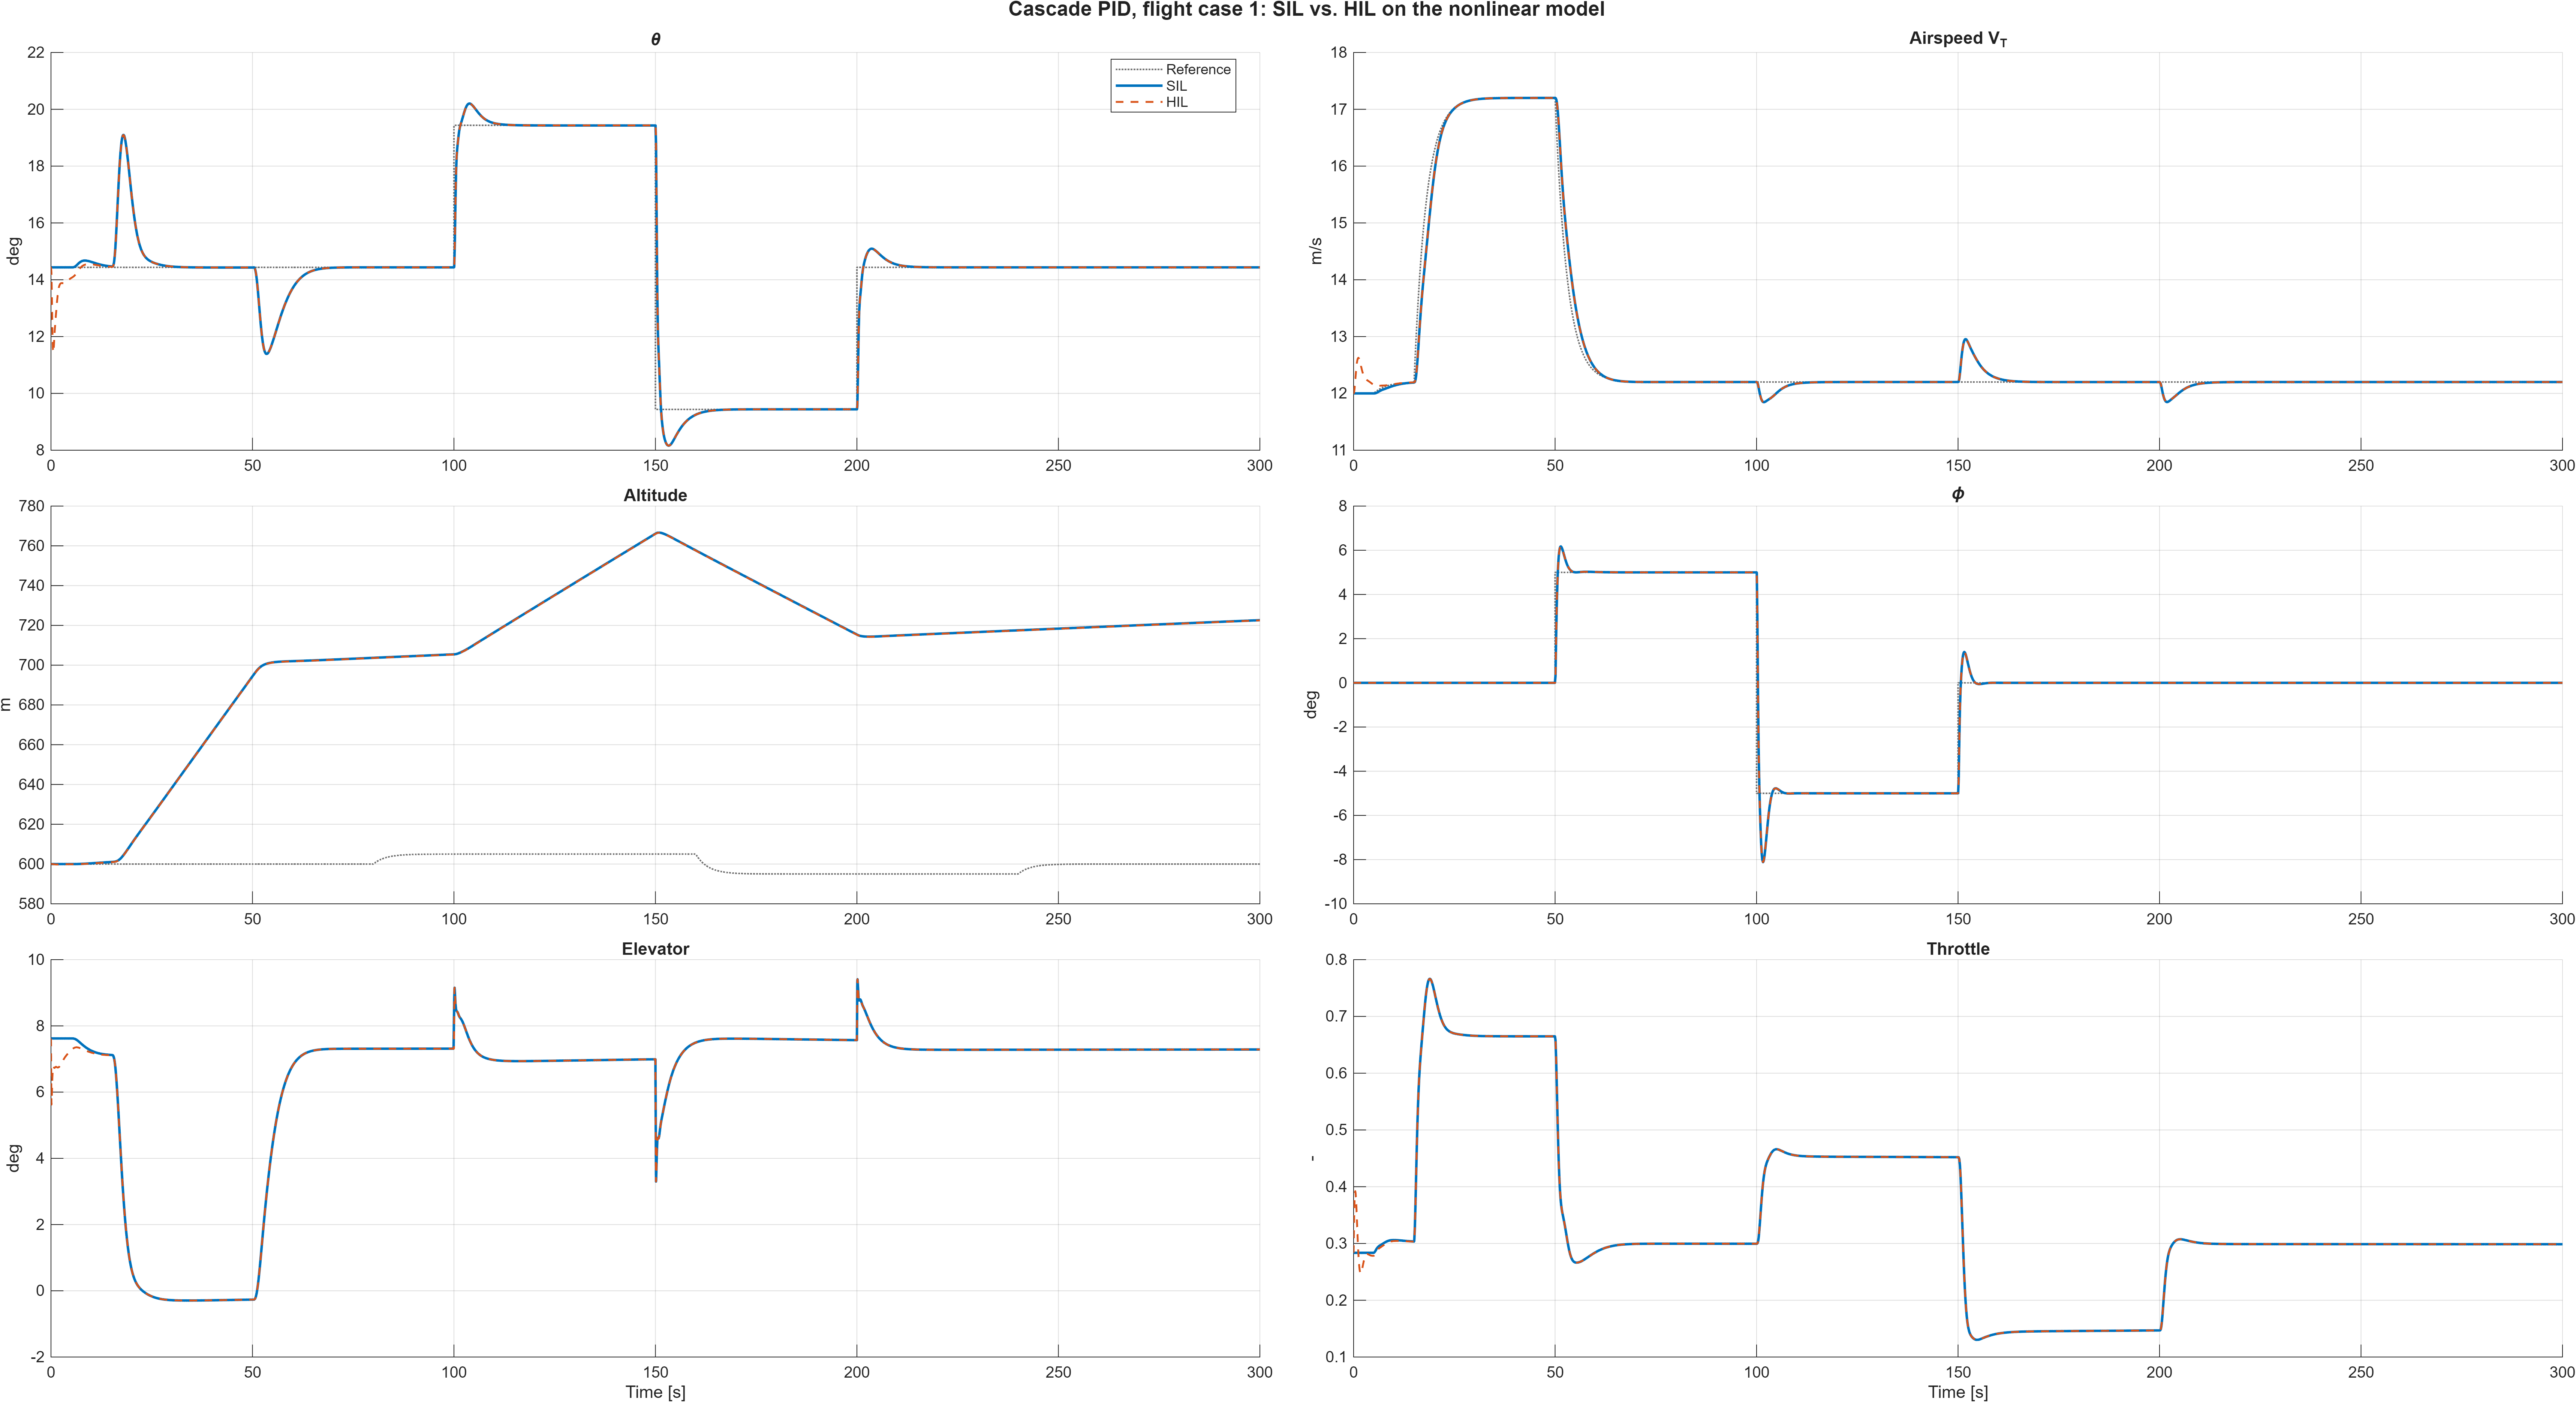
\includegraphics[width=\linewidth]{pid_sil_hil_caso1.png}
\caption{PID, flight case 1: SIL vs.\ HIL on the nonlinear model.}
\label{fig:pid-c1}
\end{figure}

\subsubsection{LQRy} The embedded LQRy is the earlier
\emph{fixed-gain} delivery --- a softer gain set than the
gain-scheduled design of Section~\ref{sec:lqry}, registered in the
repository~\cite{repo} --- so the bench results validate the
deployment pipeline for that build; re-deploying the gain-scheduled
law on the bench is future work
(Section~\ref{sec:conclusion}). The LQRy campaign was executed under the same
protocol, with per-case firmware builds and scripted programming of the
target. Its SIL--HIL residual is larger --- from $0.23^\circ$ to
$3.57^\circ$ in pitch depending on the flight case --- and is explained by
the start-up term quantified in S1: this implementation holds the
embedded integrators in reset until the link engages, so the embedded and
simulated runs begin from different states. The effect is deterministic
and confined to the transient; the doublet responses themselves track
closely.
% Figura HIL LQRy dedicada — descomentar apos regeneracao em ingles:
% \begin{figure}[!t]\centering
% \includegraphics[width=\linewidth]{fig_lqry_hil.png}
% \caption{LQRy, flight case 1: SIL vs.\ the original HIL campaign vs.\
% the corrected HIL run (SIL-sourced references, scripted flashing).}
% \label{fig:lqry-hil}\end{figure}

\subsection{Controller Comparison on the Bench}
\label{sec:fair}
With both controllers on the same bench, the same plant, the same
references, and the same metric window, the dominant free variable is
the control law --- subject to the harness asymmetries disclosed in
Section~\ref{sec:protocol}, which the equalization ablation showed not
to drive the conclusions. Fig.~\ref{fig:justo} shows flight case~1: on
the bench, the PID tracks airspeed and pitch more tightly, while the
LQRy regulates altitude better when the airspeed loop is active ---
recalling that the embedded LQRy is the earlier fixed-gain build, so
these bench observations characterize that deployment rather than the
gain-scheduled law of Section~\ref{sec:sil-comparison}.

\begin{figure}[!t]
\centering
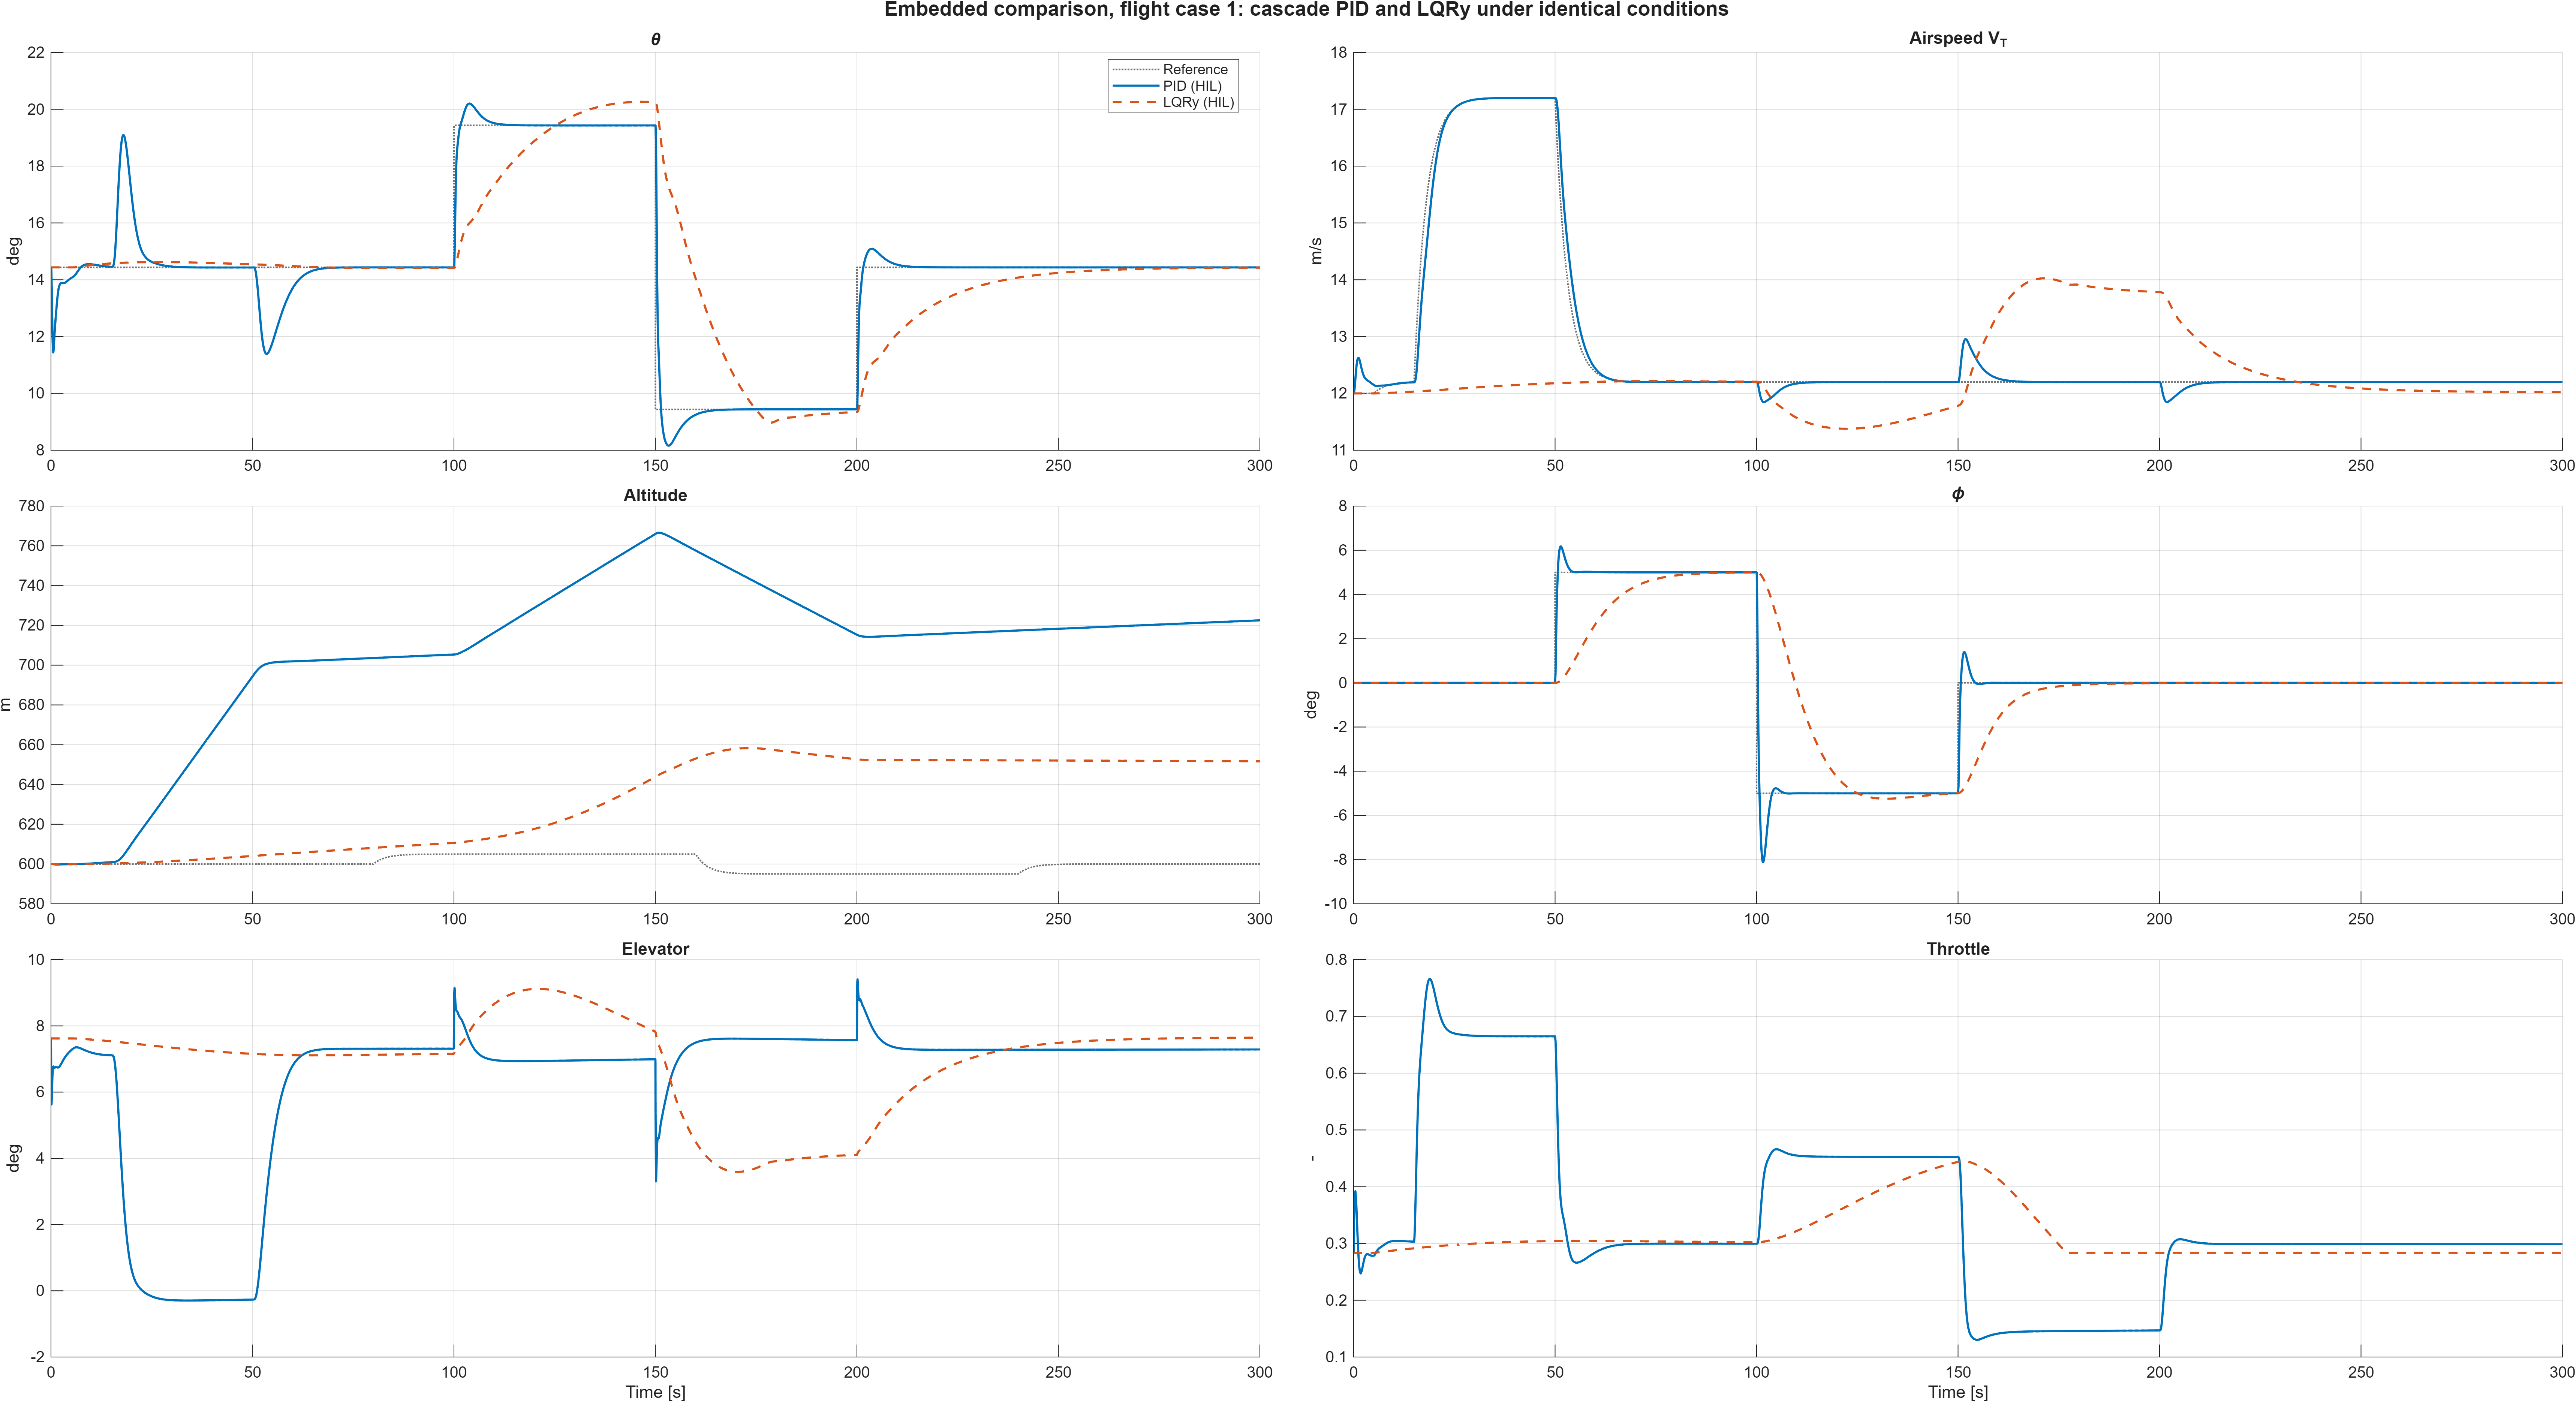
\includegraphics[width=\linewidth]{justo_caso1.png}
\caption{Embedded comparison, flight case 1: PID and LQRy under identical
conditions on the same bench.}
\label{fig:justo}
\end{figure}

\section{Conclusion}
\label{sec:conclusion}
This article covered the full path from controller design to embedded
validation for the fixed-wing flight mode of a hybrid VTOL aircraft. A
cascade PID and an output-feedback LQR were designed on the linearized
model, verified on the nonlinear model, stressed under model mismatch
and wind, and deployed to an STM32 microcontroller through automatic
code generation, so that the artifact exercised on the bench is the
production code itself.

Four results stand out. First, on the nominal plant the
requirements-retuned PID dominates the performance comparison: zero
overshoot and the tighter tracking on every guidance channel, meeting
every requirement row, while the deliberately soft fixed-gain LQRy
concedes a factor of ${\approx}5$ in airspeed RMS and violates the
airspeed-overshoot requirement ($16.5\%$). Second, the robustness
study inverts that verdict where it matters most: under a severe,
sign-changing lateral--directional model mismatch the PID loses the
mission outright, while the fixed-gain LQRy completes it with
near-nominal error --- a tolerance consistent with the classical
robustness heritage of LQ designs, earned here by the deliberately
soft tuning; the remaining scenarios add nuance: under the
longitudinal-only mismatch
the LQRy stays nominal while the PID's clamped altitude loop drifts,
under wind and gusts the PID holds every channel more tightly, and
both tolerate a plausible $+10\%$ identification uncertainty. The
comparison thus isolates a genuine performance--robustness trade-off
between the two standard laws: which one is preferable depends on
whether the dominant threat is model error --- where the PID's
failure is catastrophic and the LQRy's tolerance is decisive --- or
atmospheric disturbance, where the PID holds the line more tightly.
Third, the lockstep HIL architecture
is practically transparent when the campaign is scripted from a single
source of references and the controller start-up is synchronized: for
the synchronized PID deployment, the SIL--HIL residual reaches the
quantization floor of the communication
bus ($0.011^\circ$ in pitch attitude in the worst flight case), and the
loop is bit-deterministic --- the same generated code executed on two
different microcontroller models reproduces full 300-second flight
cases bit for bit --- which makes the bench a measuring instrument and allows a
campaign to be reproduced exactly on different hardware. Fourth,
exploiting that property, a sensitivity study ranked the implementation
choices that actually matter for SIL--HIL agreement: reference
consistency between campaigns dominates by two orders of magnitude,
start-up desynchronization leaves a persistent residual that link
quality cannot remove, low-rate frame loss is benign, and controller
discretization --- the usual first suspect --- is negligible at a
10\,ms sample rate.

Future work follows directly from the limitations identified here: a
feedforward decoupling term for the roll-to-pitch coupling quantified
in Section~\ref{sec:coupling}, evaluated on both control laws; an
extended robustness campaign with stochastic Dryden/von K\'arm\'an
turbulence~\cite{milf8785c1980,milhdbk1797} in addition to the
discrete gusts used here, and with robust syntheses designed for this
trade-off~\cite{abdulhamid2016robusto} as a third contender;
equalization of the two design harnesses (actuator models, reference
shaping, and protection logic) so that future comparisons are free of
these asymmetries; a requirements set rederived specifically for
unmanned aircraft in the sense of the scaled flying-qualities
literature~\cite{cotting2010evolution,greene2014toward};
extension of the LQRy with gain scheduling over the flight envelope,
evaluated under this same SIL-to-HIL protocol; and flight
testing of the embedded controllers validated on the bench, closing
the simulation-to-flight loop that the HIL stage
approximates~\cite{shen2025model}.


\bibliographystyle{IEEEtran}
\bibliography{refs}

% ---- Biografias (IEEE Access exige; fotos 1in x 1.25in) ----
% PENDENTE-EXTERNO: dados biograficos reais + fotos dos tres autores.
% Estrutura pronta abaixo; completar antes da submissao.
\begin{biography}{Kau\^e Martins}
is with the Electronic Devices and Systems area (EEC-D) of the
Instituto Tecnol\'ogico de Aeron\'autica (ITA), S\~ao Jos\'e dos
Campos, Brazil. % PENDENTE-EXTERNO: titulacao, ano, interesses.
\end{biography}

\begin{biography}{Huascar Mirko Montecinos Cortez}
is with the Electronic Devices and Systems area (EEC-D) of the
Instituto Tecnol\'ogico de Aeron\'autica (ITA), S\~ao Jos\'e dos
Campos, Brazil. % PENDENTE-EXTERNO: titulacao, ano, interesses.
\end{biography}

\begin{biography}{Neusa Maria Franco de Oliveira}
is a professor with the Instituto Tecnol\'ogico de Aeron\'autica
(ITA), S\~ao Jos\'e dos Campos, Brazil, where she advises research on
unmanned aerial vehicle identification, control, and
hardware-in-the-loop validation.
% PENDENTE-EXTERNO: titulacao, historico, interesses completos.
\end{biography}

\EOD
\end{document}
